\section{Comportement}
\label{sec:Comportement}
	Concernant les blessures préalablement observées sur les souris \mcrd mâles lors du stage de B. SOMON, elles n'ont pas pu être reproduites durant mon stage. Les animaux (mutants comme hétérozygotes) ont cependant été qualifiés de "plus sensible à leurs environnement que la normale" par les animaliers en charges de ceux-ci. Comme durant le stage de B. Somon, les animaux n'étaient pas situés dans la même animalerie qu'actuellement (zone sanctuaire de l'ICM et zone EOPS de l'animalerie de Paris Descartes), on peut émettre l'hypothèse que les souris étaient soumises à un stress plus important, qui expliquerait un comportement d'automutilation/hypergrooming chez les souris mutantes. 
	%\todo{Resultats Laure strochlic + maze test}

\section{Structure du cerveau}
\label{sec:NisslResultat}
	La coloration de Nissl, ici à base de Crésyl violet, est un marquage classique du tissu nerveux avec une molécule basique, qui marque particulièrement l'acide nucléique (\acrshort{adn} et \acrshort{arn}) des cellules car basophile (ces structures au microscope prennent le nom de "Corps de Nissl'). Ce marquage est important dans les neurones, riches en \gls{re} rugueux, organite associé à une grande quantité d'\acrshort{arn}. Cette coloration permet ainsi de visualiser les différentes structures cellulaires au sein du tissu nerveux.

	Comme les protéines \gls{wnt} sont généralement impliquées dans le développement et l'organisation du cerveau, on peut alors se demander si la suppression du domaine de liaisons de ces protéines sur le récepteur \gls{musk} allait entraîner des modifications du développement du système nerveux qui serait visible avec une coloration histologique.

	Afin de comparer l'organisation structurale du cerveau chez la souris sauvage et mutante, une coloration de Nissl a donc été réalisée sur 4 individus : 2 souris mutantes et 2 souris sauvages (1 mâle et 1 femelle pour chaque groupe) (\cref{fig:NisslResultat}). Ce marquage a donc permis de mettre en évidence que la mutation de \gls{musk} ne modifiait pas l'organisation du cerveau, à la fois chez les souris femelles (\cref{fig:FemWTNissl,fig:FemMutNissl}) et mâles (\cref{fig:MaleWTNissl,fig:MaleMutNissl}). 

	\begin{figure}[h] %Figure Nissl Résultats
		\begin{center}
			\begin{subfigure}[h]{0.49\textwidth}%F437 WT Nissl 33 l2.tif
				\caption{}
				\label{fig:FemWTNissl}
				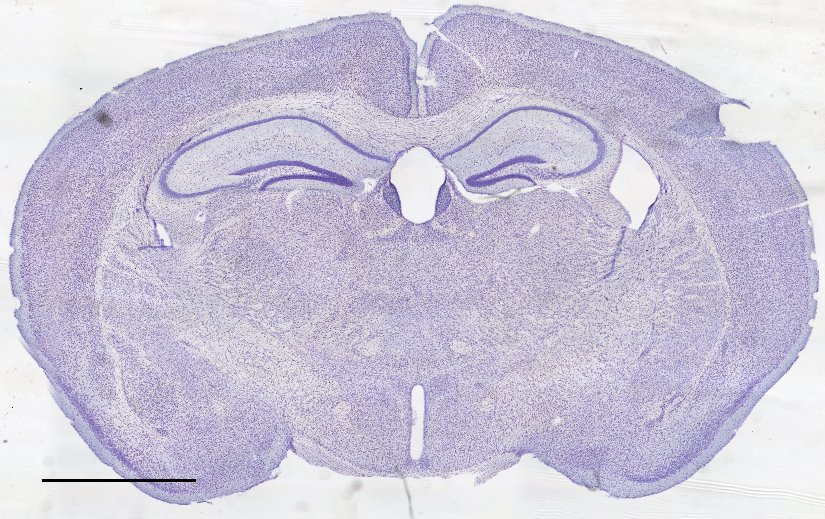
\includegraphics[width=\textwidth]{./Images/Nissl/FemWT.jpg}
			\end{subfigure}
			\begin{subfigure}[h]{0.49\textwidth}%F435 Mut Nissl 38.tif
				\caption{}
				\label{fig:FemMutNissl}
				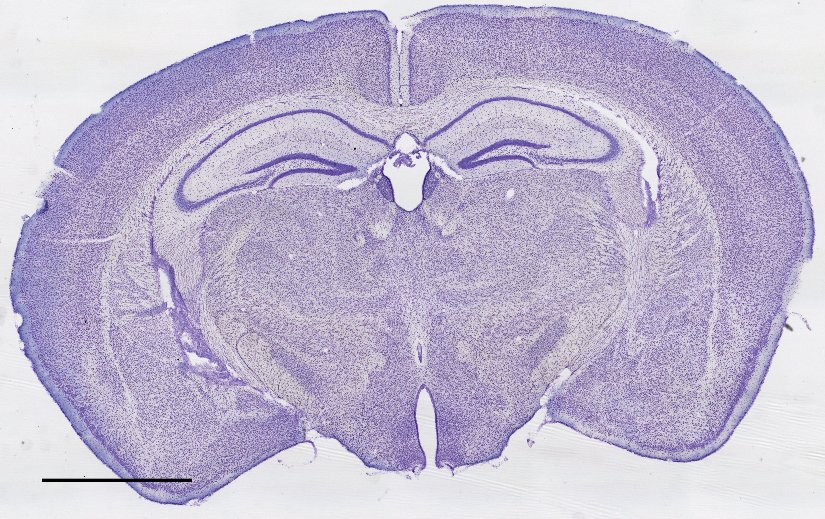
\includegraphics[width=\textwidth]{./Images/Nissl/FemMut.jpg}
			\end{subfigure}
			\begin{subfigure}[h]{0.49\textwidth}%M2 WT Nissl #031.tif
				\caption{}
				\label{fig:MaleWTNissl}
				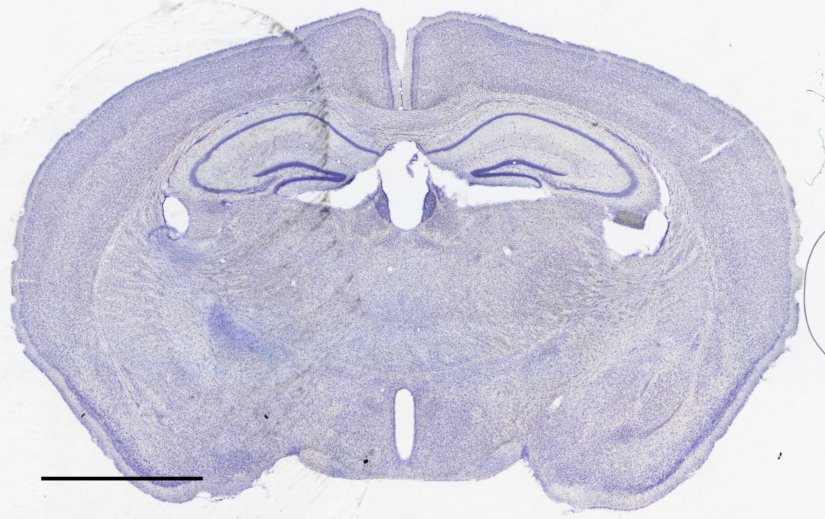
\includegraphics[width=\textwidth]{./Images/Nissl/MaleWT.jpg}
			\end{subfigure}
			\begin{subfigure}[h]{0.49\textwidth}%M442 Mut Nissl lame 3 36.tif
				\caption{}
				\label{fig:MaleMutNissl}
				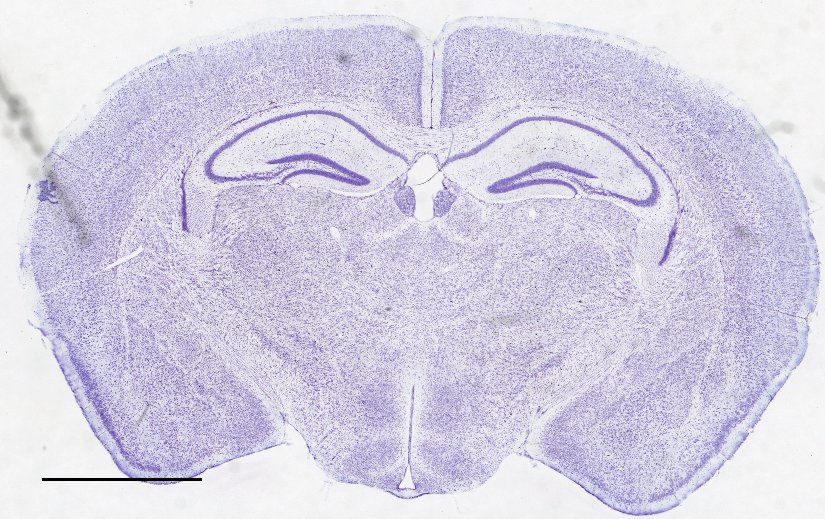
\includegraphics[width=\textwidth]{./Images/Nissl/MaleMut.jpg}
			\end{subfigure}
		\end{center}
		\caption{Les souris \mcrd ne présentent pas de défauts de structure du \acrshort{snc}.}
		\descfig{%
			Coloration de Nissl sur : 
			\subref{fig:FemWTNissl} Femelle sauvage, 
			\subref{fig:FemMutNissl} Femelle mutante, 
			\subref{fig:MaleWTNissl} Mâle sauvage, 
			\subref{fig:MaleMutNissl} Mâle mutant. 
			Images représentatives de coupes réalisées au niveau de l'hippocampe. 
			Âge moyen des souris : 30 jours. 
			Barre d'échelle : 2 mm.
				}
		\label{fig:NisslResultat}
	\end{figure}
	\FloatBarrier

\section{Distribution des neurones dans le cerveau}
	\label{sec:neun}
	Pour visualiser l'organisation des neurones dans l'hippocampe des souris mutantes, j'ai révélé les neurones par \acrshort{ihc} en utilisant des anticorps dirigés contre \acrshort{neun}. \Acrshort{neun} (connu aussi sous le nom de Fox-3) est un marqueur du  corps cellulaire et des noyaux de presque tout les neurones, couramment utilisé \cite{Guselnikova2015, Kim2009}. 
	
	Grâce à des mesures d'épaisseur de la couche pyramidale (CA1, CA3) et granulaire (Gyrus Denté) réalisées dans différentes régions de l'hippocampe sur des coupes rostrale, médiane et caudale, il apparaît que la structure de l'hippocampe est modifiée chez les souris mutantes par rapport aux souris sauvages (\cref{fig:NeuNResultat}). En comparant les mesures des coupes rostrale, il y a une différence dans la région du Gyrus Denté (72.5$\pm$18.17µm (\acrshort{wt}) vs 57.3$\pm$13.84µm (mutant), p-value : 0.0138) (\cref{fig:NeunQuantifNasal}).  Au niveau de coupes médiane, aucune différences ne ressort des différentes mesures effectuées (\cref{fig:NeunQuantifMilieu}). Pour les coupes caudale, on peut observer une différences d'épaisseur de la couche entre les souris \gls{wt} et \mcrd dans la région CA3 (111.2$\pm$78.39µm (\acrshort{wt}) vs 78.39$\pm$39.22 (mutant), p-value : 0.0129), et les deux sous-région du Gyrus denté (DG1 : 50.29$\pm$9.655 (\acrshort{wt}) vs 63.44$\pm$17.37 (mutant), p-value : 0.0244 ; et DG2 : 61.29$\pm$10.24 (\acrshort{wt}) vs 51.78$\pm$12.46 (mutant), p-value : 0.0367)(\cref{fig:NeunQuantifPost}).
	
	\begin{figure}[h]
		\begin{subfigure}[h]{0.329\textwidth} %M2 WT NeuN 3.tiff
			\caption{}
			\label{fig:NeuNIllu1}
			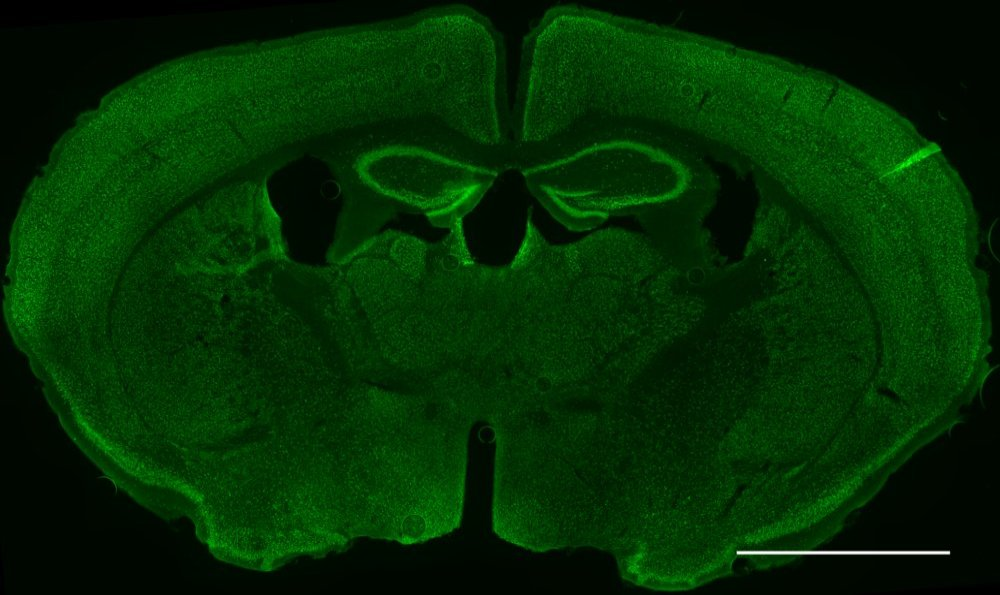
\includegraphics[width=\textwidth]{./Images/Immuno/NeuN/M2WT_NeuN_10x_1.jpg}
		\end{subfigure}
		\begin{subfigure}[h]{0.329\textwidth} %M2 WT NeuN 5.tiff
			\caption{}
			\label{fig:NeuNIllu2}
			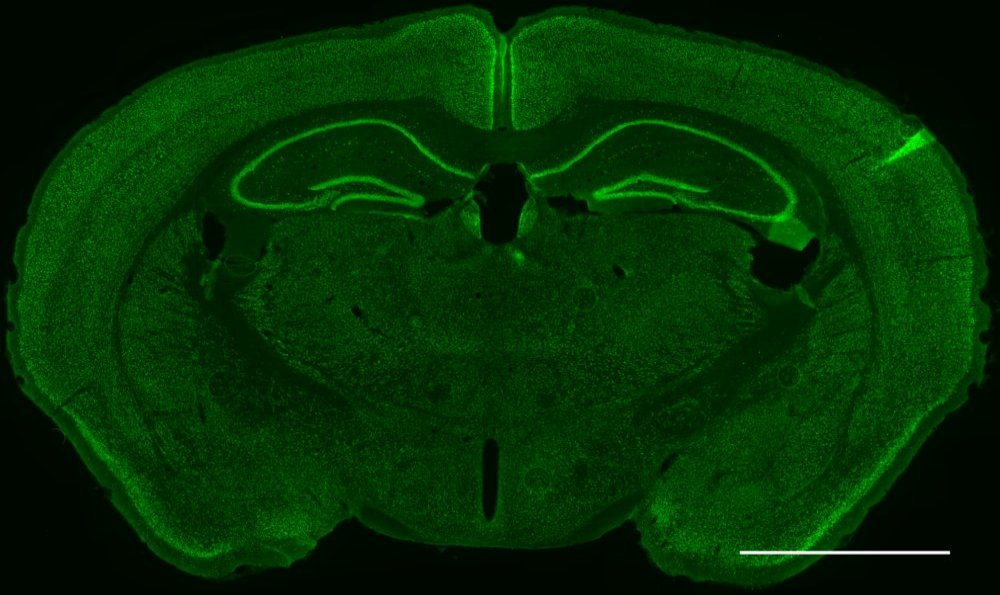
\includegraphics[width=\textwidth]{./Images/Immuno/NeuN/M2WT_NeuN_10x_2.jpg}
		\end{subfigure}
		\begin{subfigure}[h]{0.329\textwidth} %M2 WT NeuN 7.tiff
			\caption{}
			\label{fig:NeuNIllu3}
			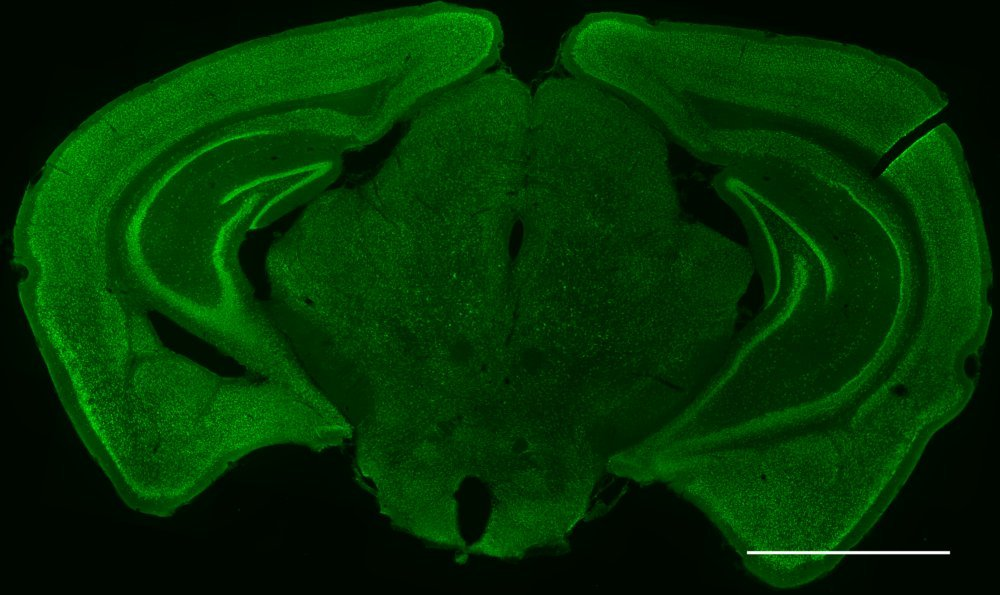
\includegraphics[width=\textwidth]{./Images/Immuno/NeuN/M2WT_NeuN_10x_3.jpg}
		\end{subfigure}
		\begin{subfigure}[h]{0.329\textwidth}
			\caption{}
			\label{fig:hippIllu}
			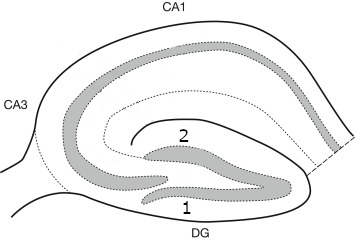
\includegraphics[width=\textwidth]{./Images/HippSchema.jpg}
		\end{subfigure}
		\begin{subfigure}[h]{0.329\textwidth}
			\caption{}
			\label{fig:NeunQuantifNasal}
			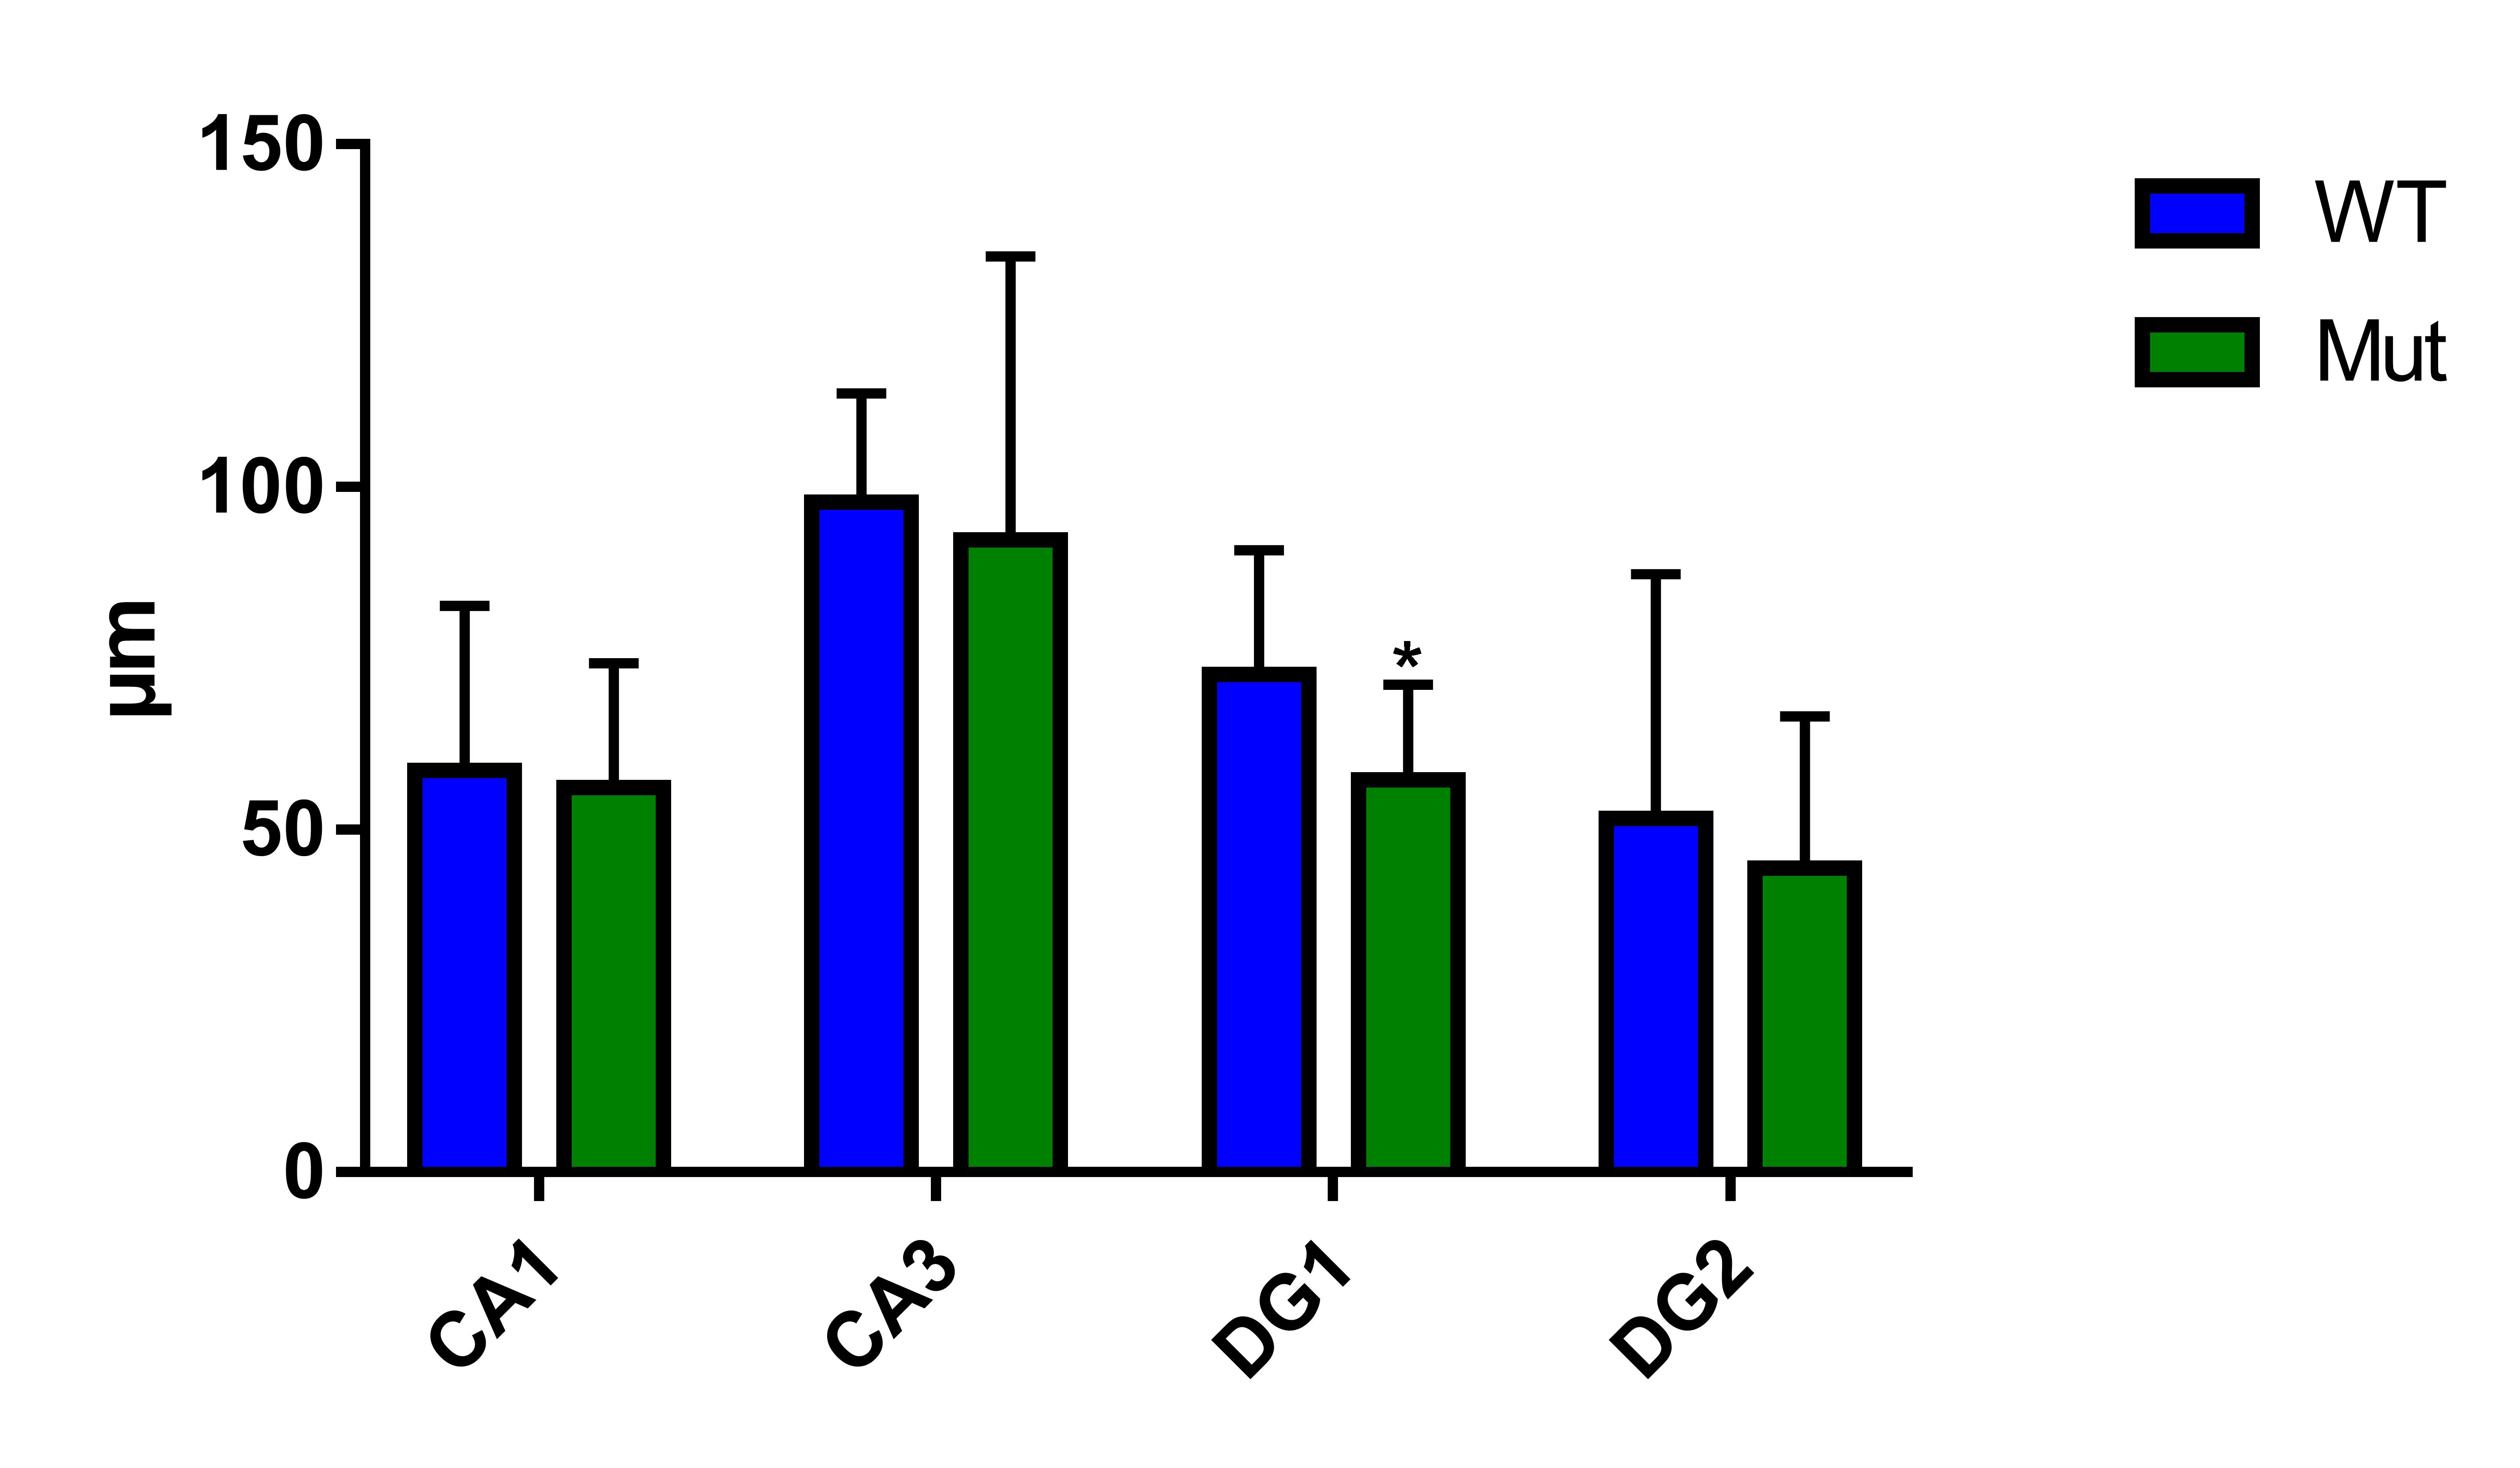
\includegraphics[width=\textwidth]{./Images/Immuno/NeuN/Quantif_Nasal.jpg}
		\end{subfigure}
		\begin{subfigure}[h]{0.329\textwidth}
			\caption{}
			\label{fig:NeunQuantifMilieu}
			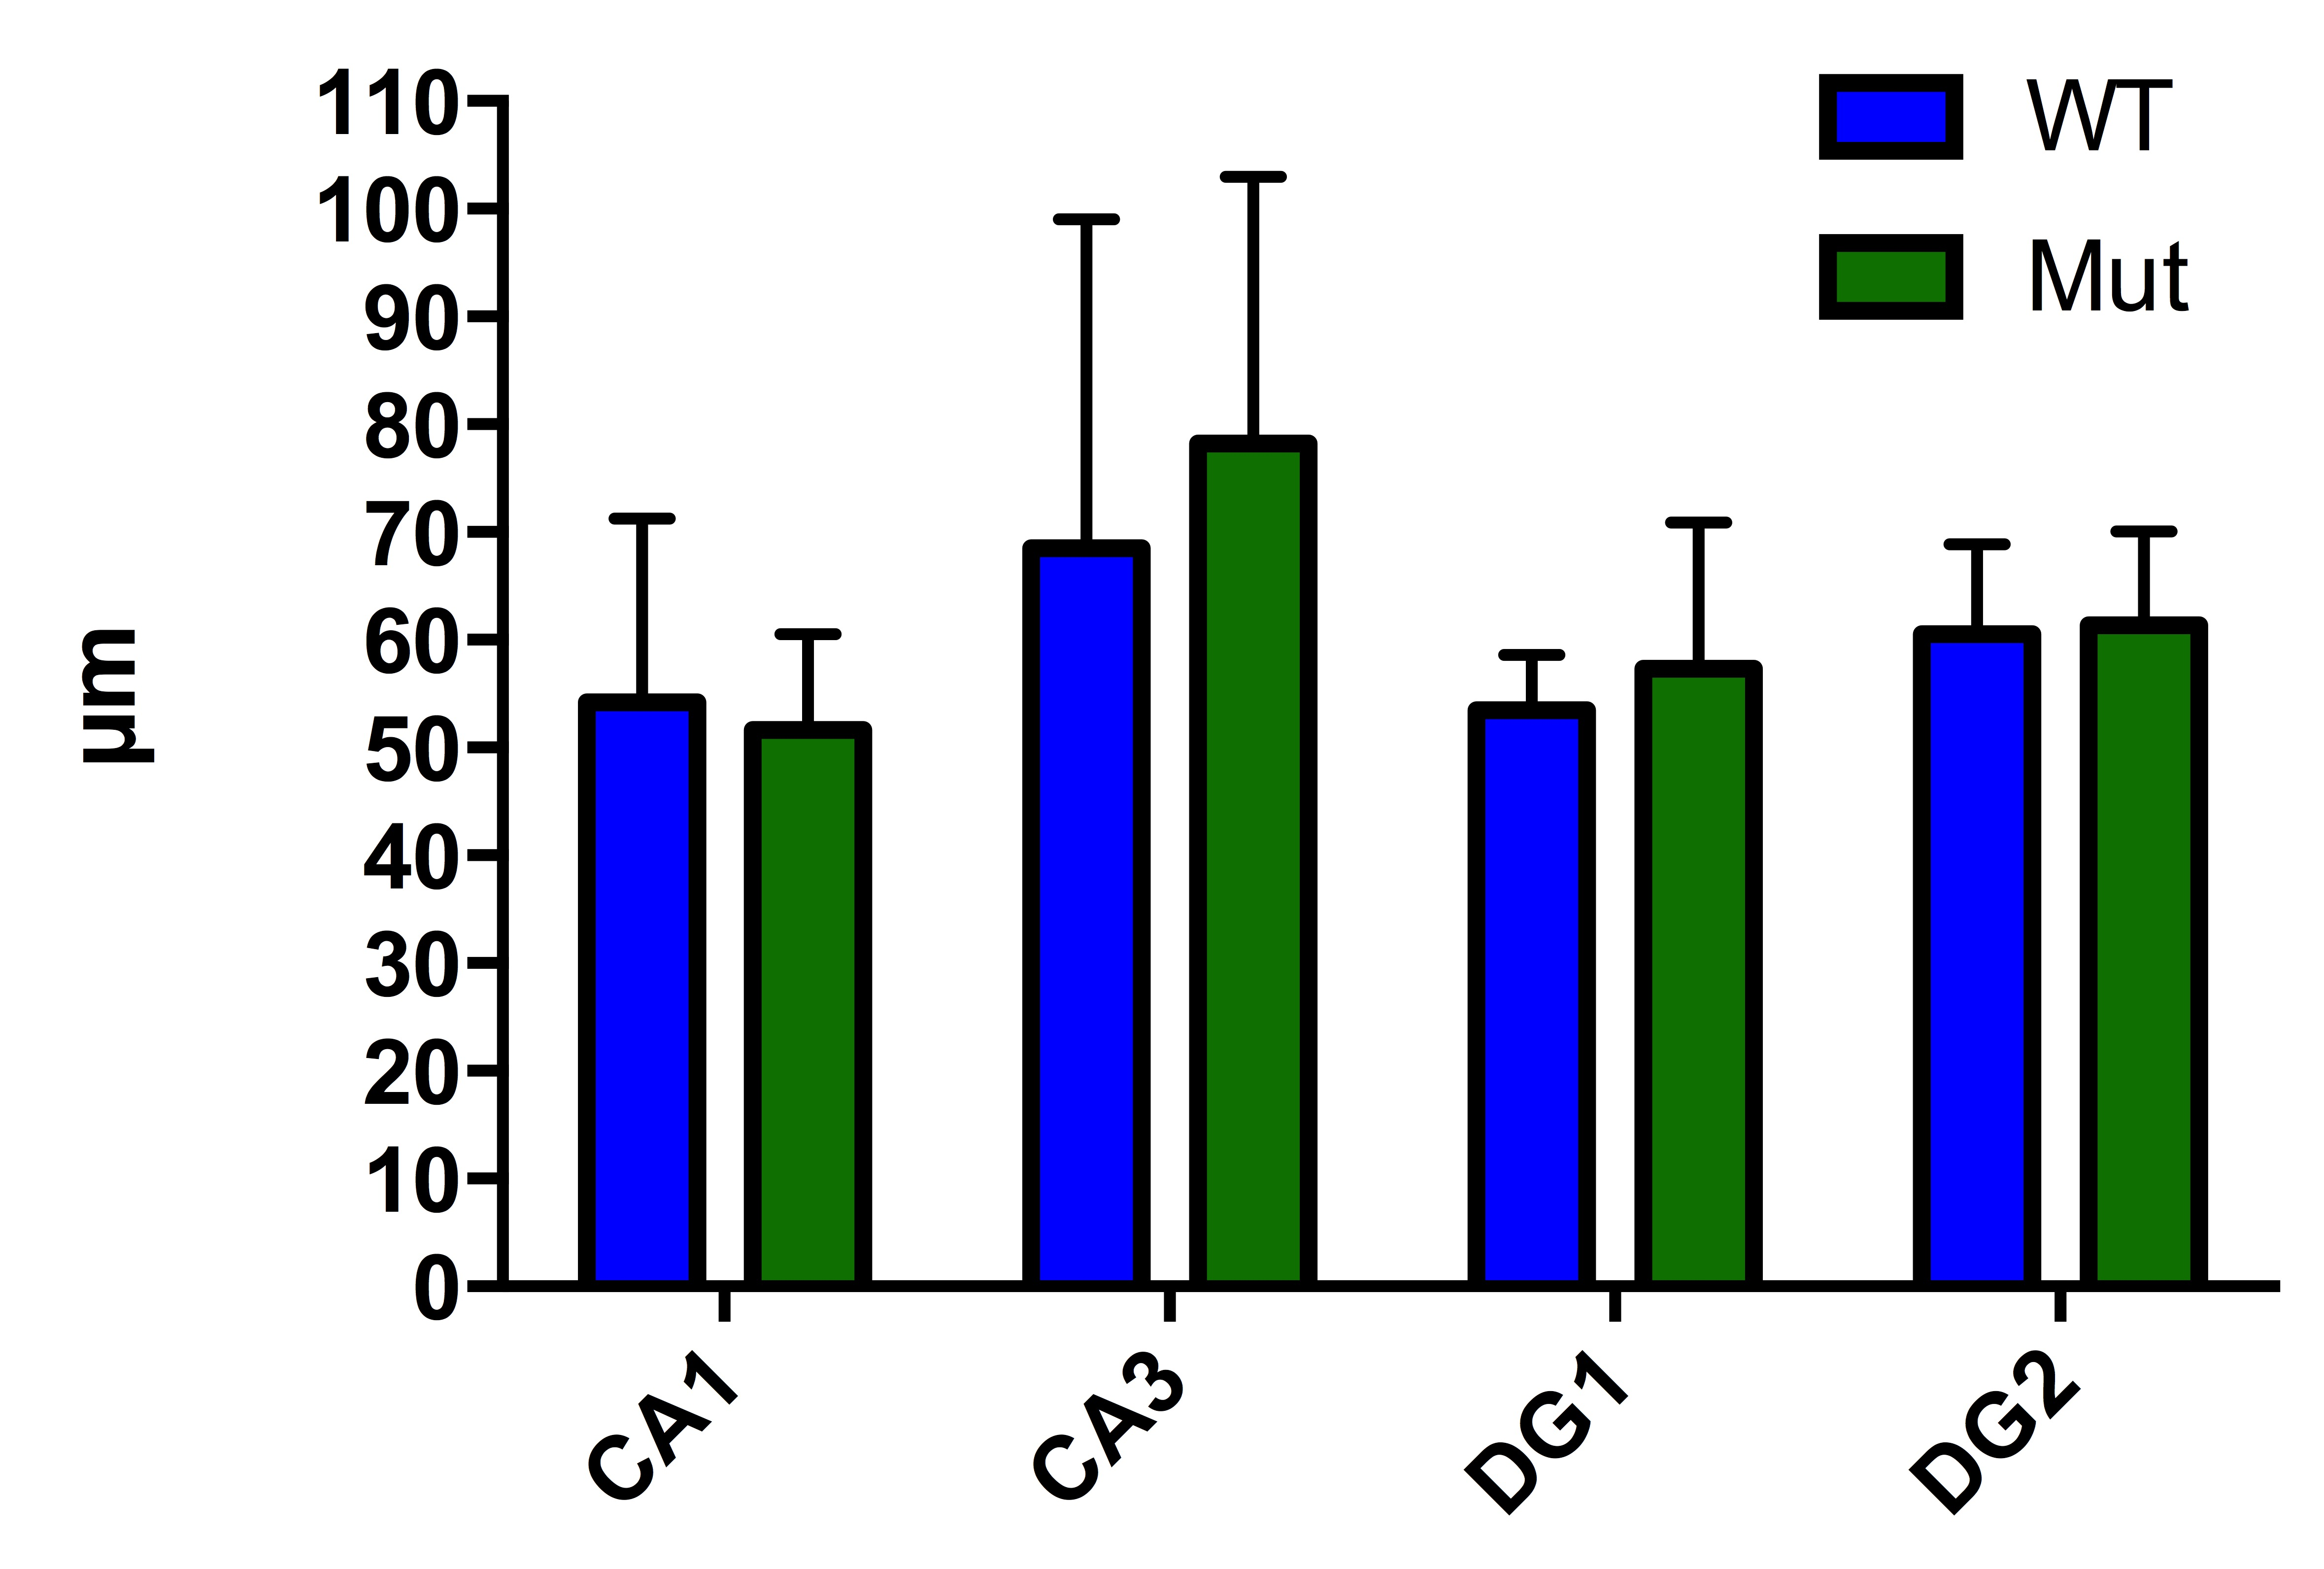
\includegraphics[width=\textwidth]{./Images/Immuno/NeuN/Quantif_Milieu.jpg}
		\end{subfigure}
		\begin{subfigure}[h]{0.329\textwidth}
			\caption{}
			\label{fig:NeunQuantifPost}
			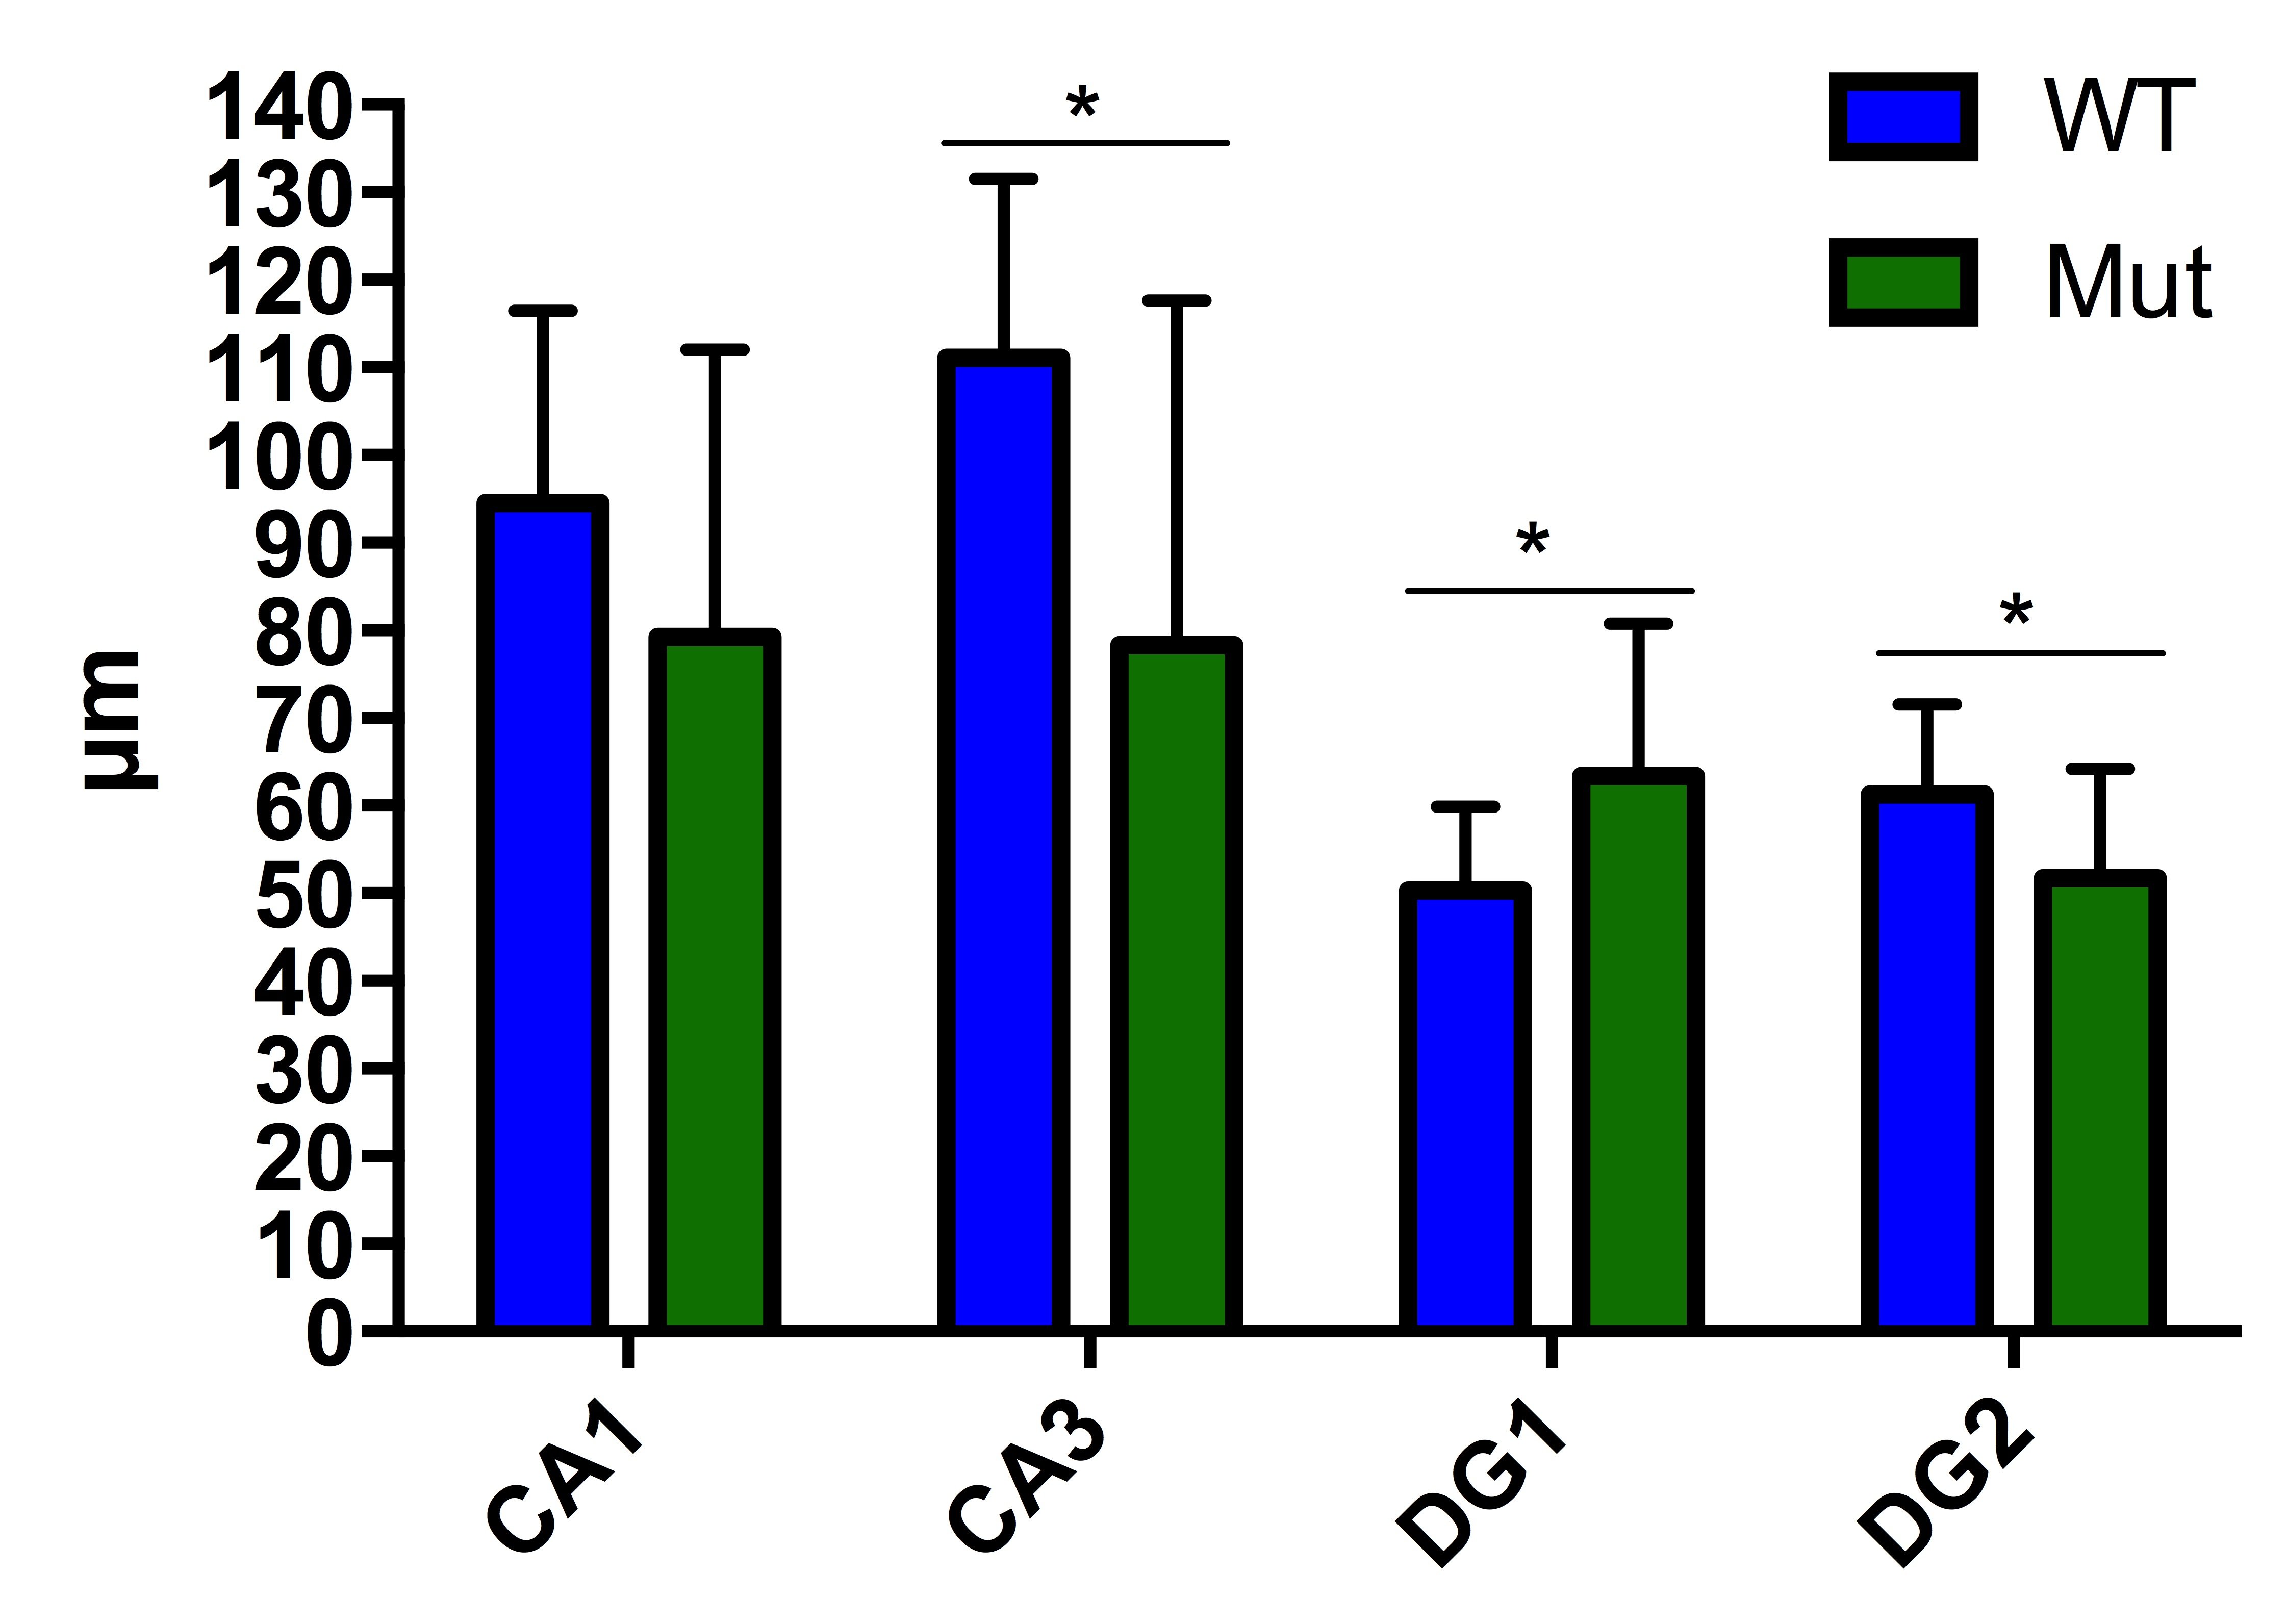
\includegraphics[width=\textwidth]{./Images/Immuno/NeuN/Qantif_Post.jpg}
		\end{subfigure}
		\caption{L'organisation de l'hippocampe est modifié par la mutation \mcrd.}
		\descfig{%
				Marquage de \acrshort{neun} sur tranche de cerveau. Illustration des différentes profondeurs choisies pour les mesures.
				\subref{fig:NeuNIllu1} Exemple de coupe rostrale.
				\subref{fig:NeuNIllu2} Exemple de coupe médiane.
				\subref{fig:NeuNIllu3} Exemple de coupe caudale.
				\subref{fig:hippIllu} Illustration des régions CA1, CA3, et DG 1\&2 où sont effectuées les mesures. Issue de Li et Pleasure, 2013 \cite{Li2013a}.
				\subref{fig:NeunQuantifNasal} Quantification de l'épaisseur de la couche pyramidale de différentes régions de l'hippocampe sur des coupes rostrales. 
				\subref{fig:NeunQuantifMilieu} Quantification sur des coupes médianes.
				\subref{fig:NeunQuantifPost} Quantification sur des coupes caudales.
				Ca : Cornus Ammonis, DG : Gyrus Denté. 
				Barre d'échelle : 2mm. 
				Test statistique : Test t de Student non apparié. 
				* : p<0.05, ** : p<0.01, *** : p<0.001. 
				n = 2 (\acrshort{wt}) et n = 3 (mutants).
				}
		\label{fig:NeuNResultat}
	\end{figure}
\FloatBarrier
	
\section{Localisation et identification des cellules neurales exprimant \acrshort{musk}}
	\label{ssec:musk}
	Après avoir observé l'organisation globale et neuronale du cerveau de souris, j'ai cherché à identifier les régions du cerveau exprimant \gls{musk}. Pour cela, j'ai eu recours à une technique d'immunohistochimie. L'anticorps utilisé est un anticorps polyclonal de lapin, dirigé contre le domaine extracellulaire de \gls{musk} (information donnée par le fournisseur).
	
	Malgré le fait que le niveau d'expression de \gls{musk} soit considéré comme faible dans le tissu nerveux d'après des études antérieurs (par northen blot principalement), j'ai quand même pu observé un marquage de cette protéine dans diverses régions discrètes du cerveau : Hippocampe (couche radiaire et moléculaire principalement) (\cref{fig:locaMuSKca1}), Corps calleux (\cref{fig:locaMuSKcc}), Habenula médiale (\cref{fig:locaMuSKhb}), Fasciculus retroflexus (\cref{fig:locaMuSKfr}), Capsule interne, Noyau caudé, 3ème ventricule ventrale, Cervelet principalement (\cref{fig:ImmunoMusk}). 
	
	%\todo{Ajouter zoom, faire menage bruit de fond}
	\begin{figure}[h] %Figure Immuno MuSK Résultats
		\begin{subfigure}[h]{0.99\textwidth}
			\caption{}
			\label{fig:locaMusK}
			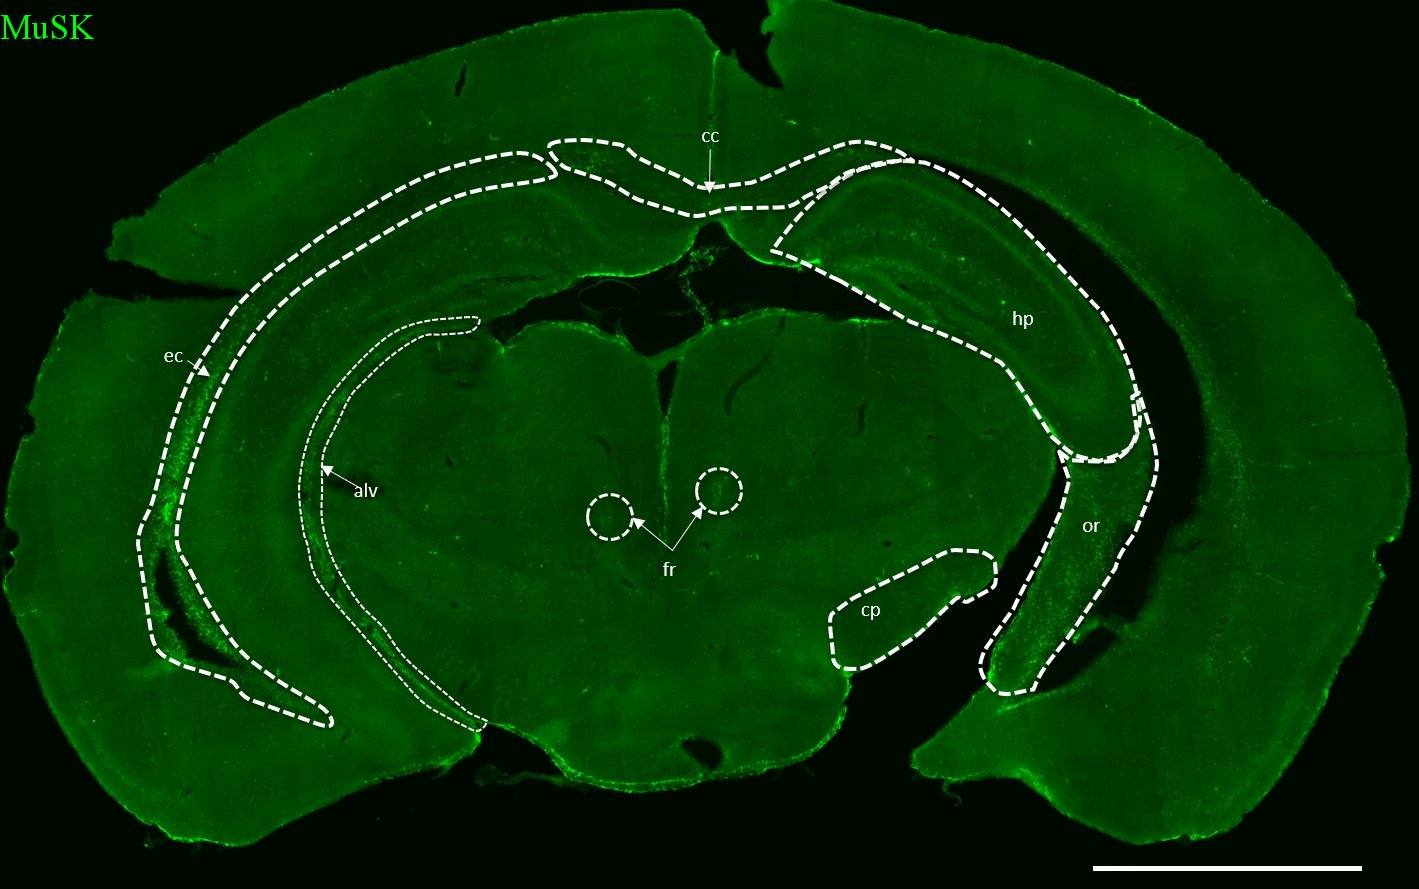
\includegraphics[width=\textwidth]{./Images/Immuno/Musk/loca_MuSK.jpg}
		\end{subfigure}
		\begin{subfigure}[h]{0.245\textwidth}
			\caption{}
			\label{fig:locaMuSKcc}
			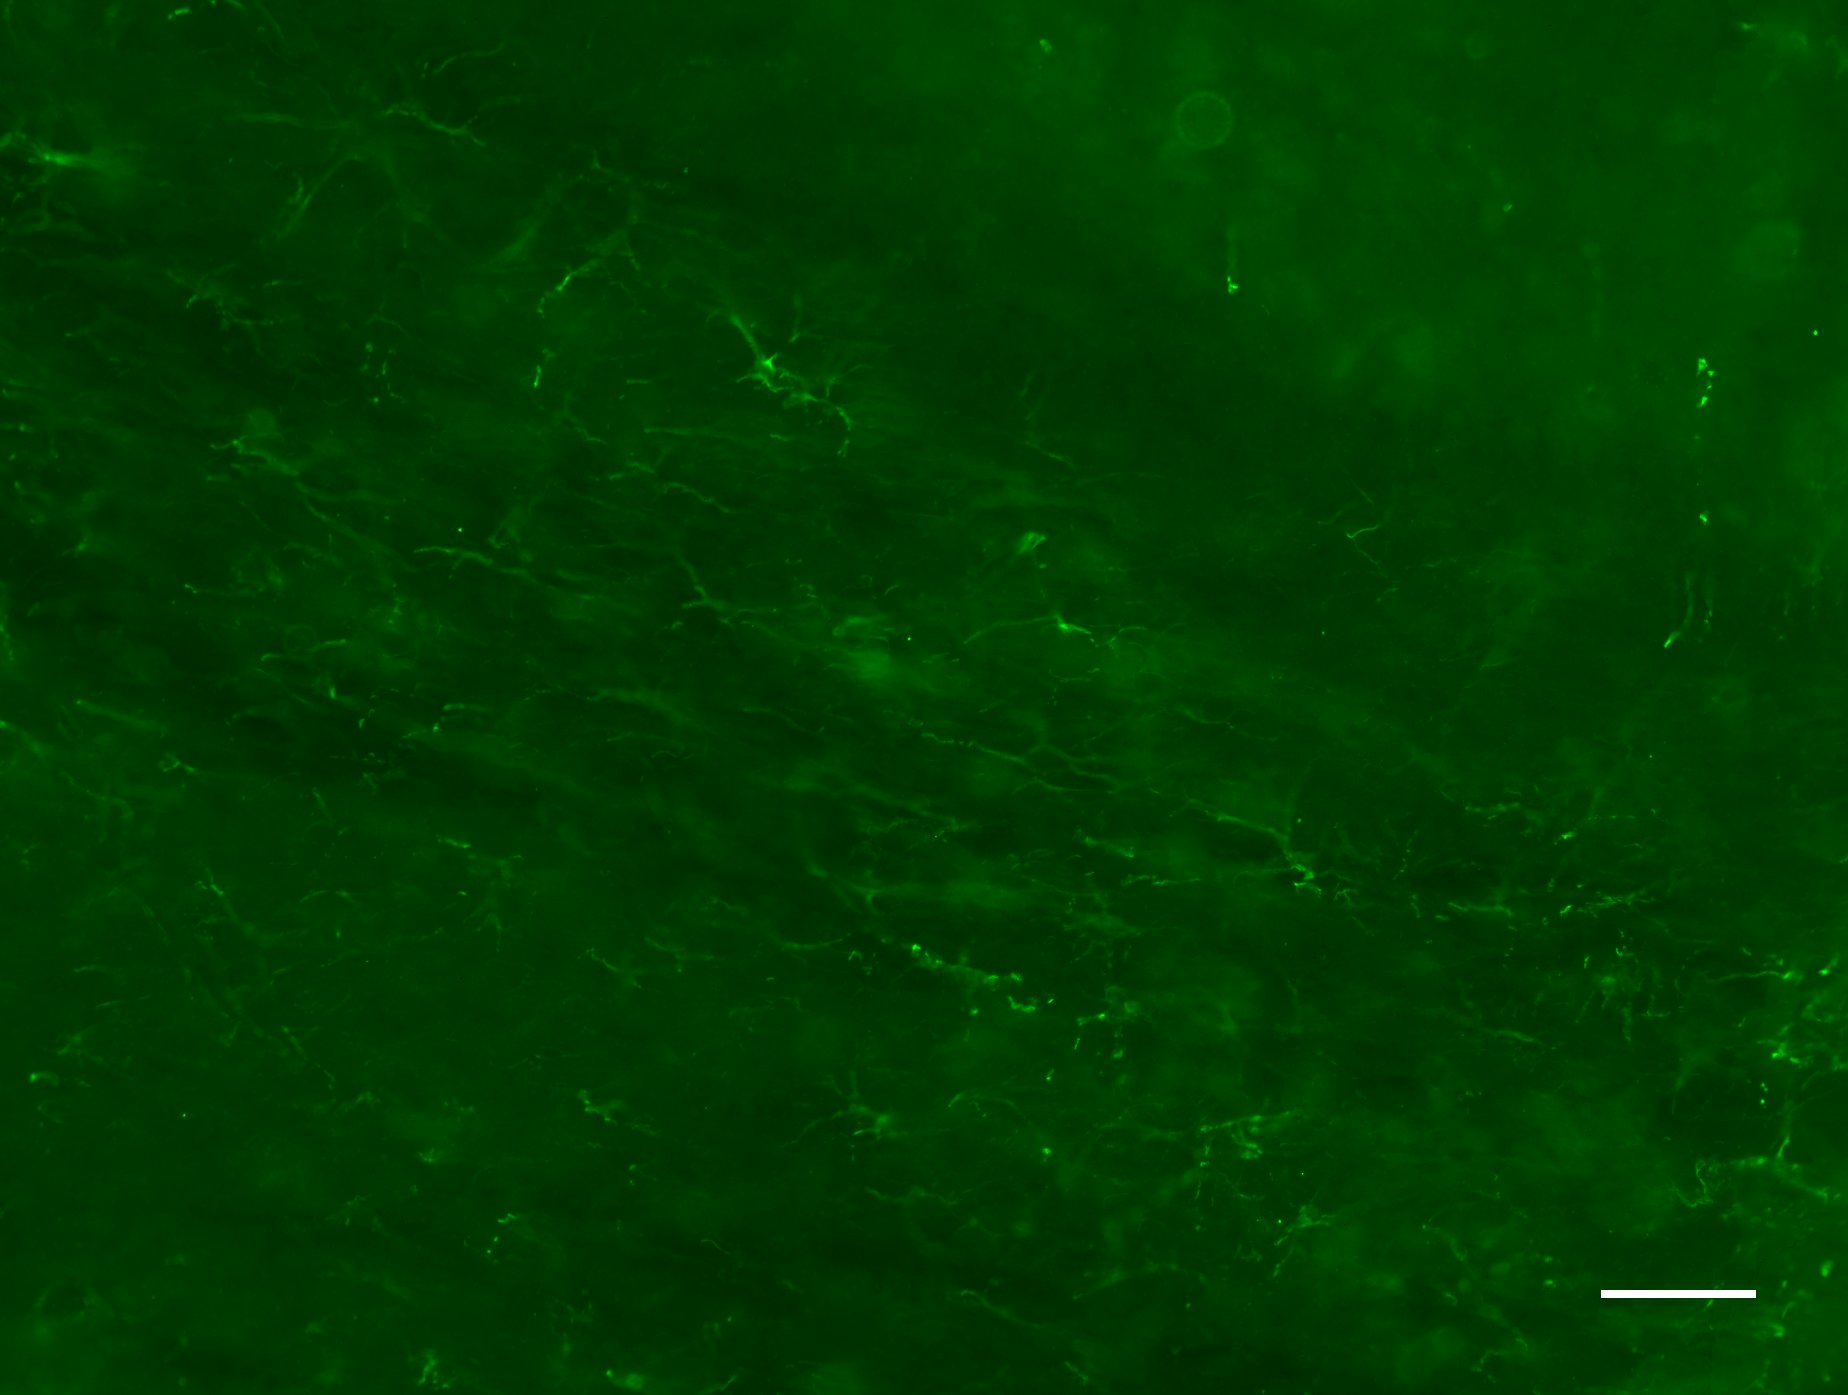
\includegraphics[width=\textwidth]{./Images/Immuno/Musk/MuSK_cc_50um.jpg}
		\end{subfigure}
		\begin{subfigure}[h]{0.245\textwidth}
			\caption{}
			\label{fig:locaMuSKca1}
			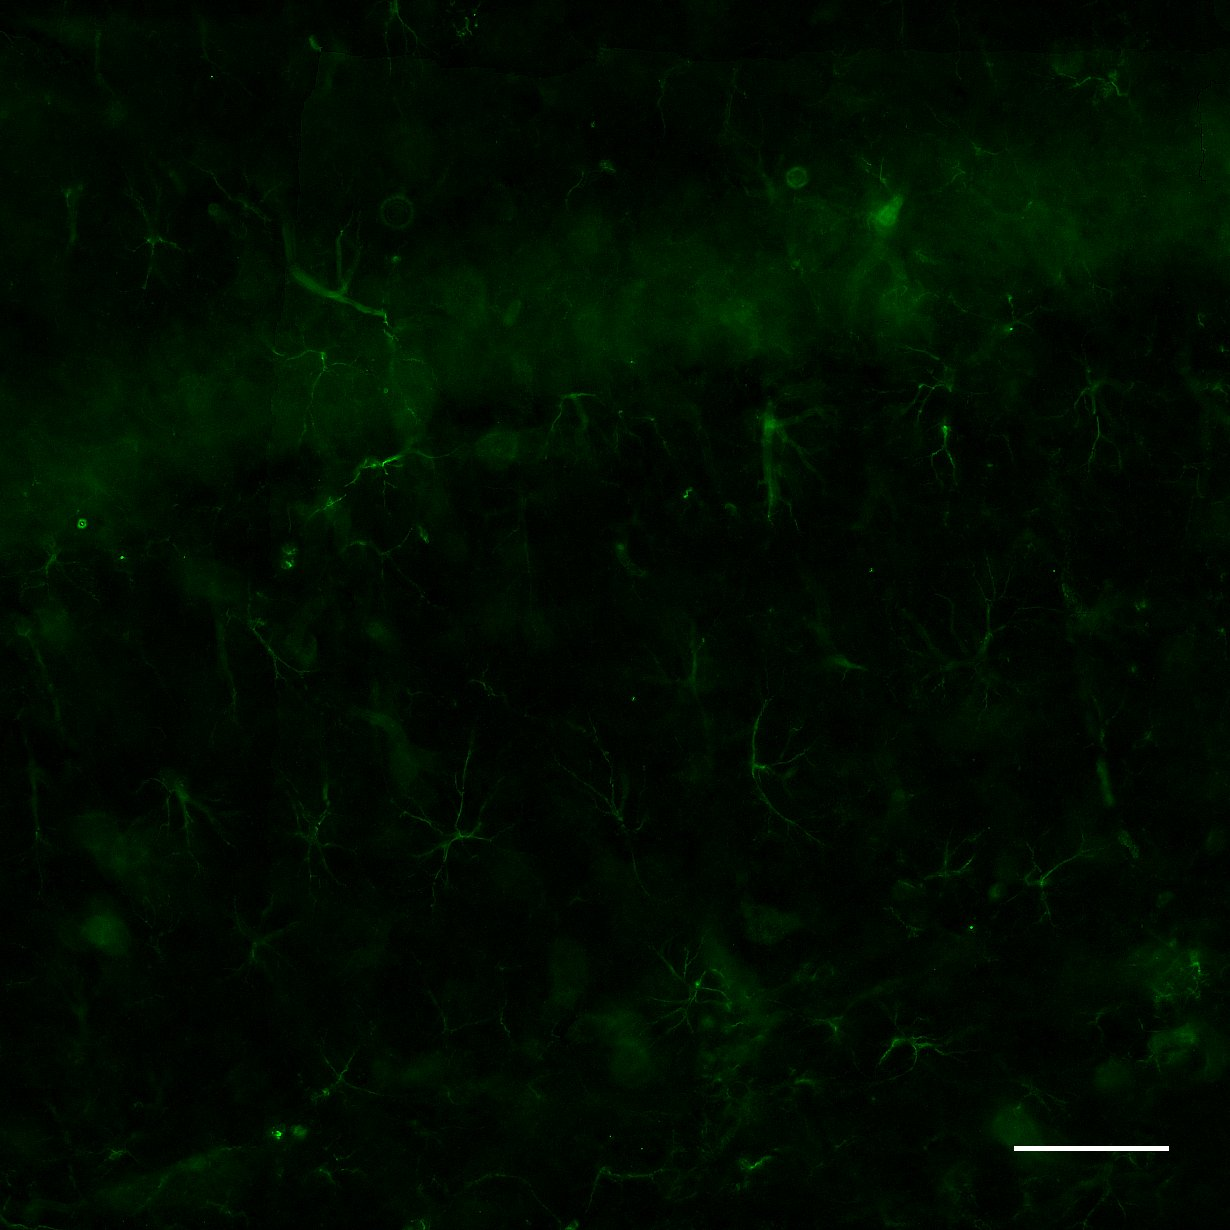
\includegraphics[width=\textwidth]{./Images/Immuno/Musk/MuSK_ca1_50um.jpg}
		\end{subfigure}
		\begin{subfigure}[h]{0.245\textwidth}
			\caption{}
			\label{fig:locaMuSKdg}
			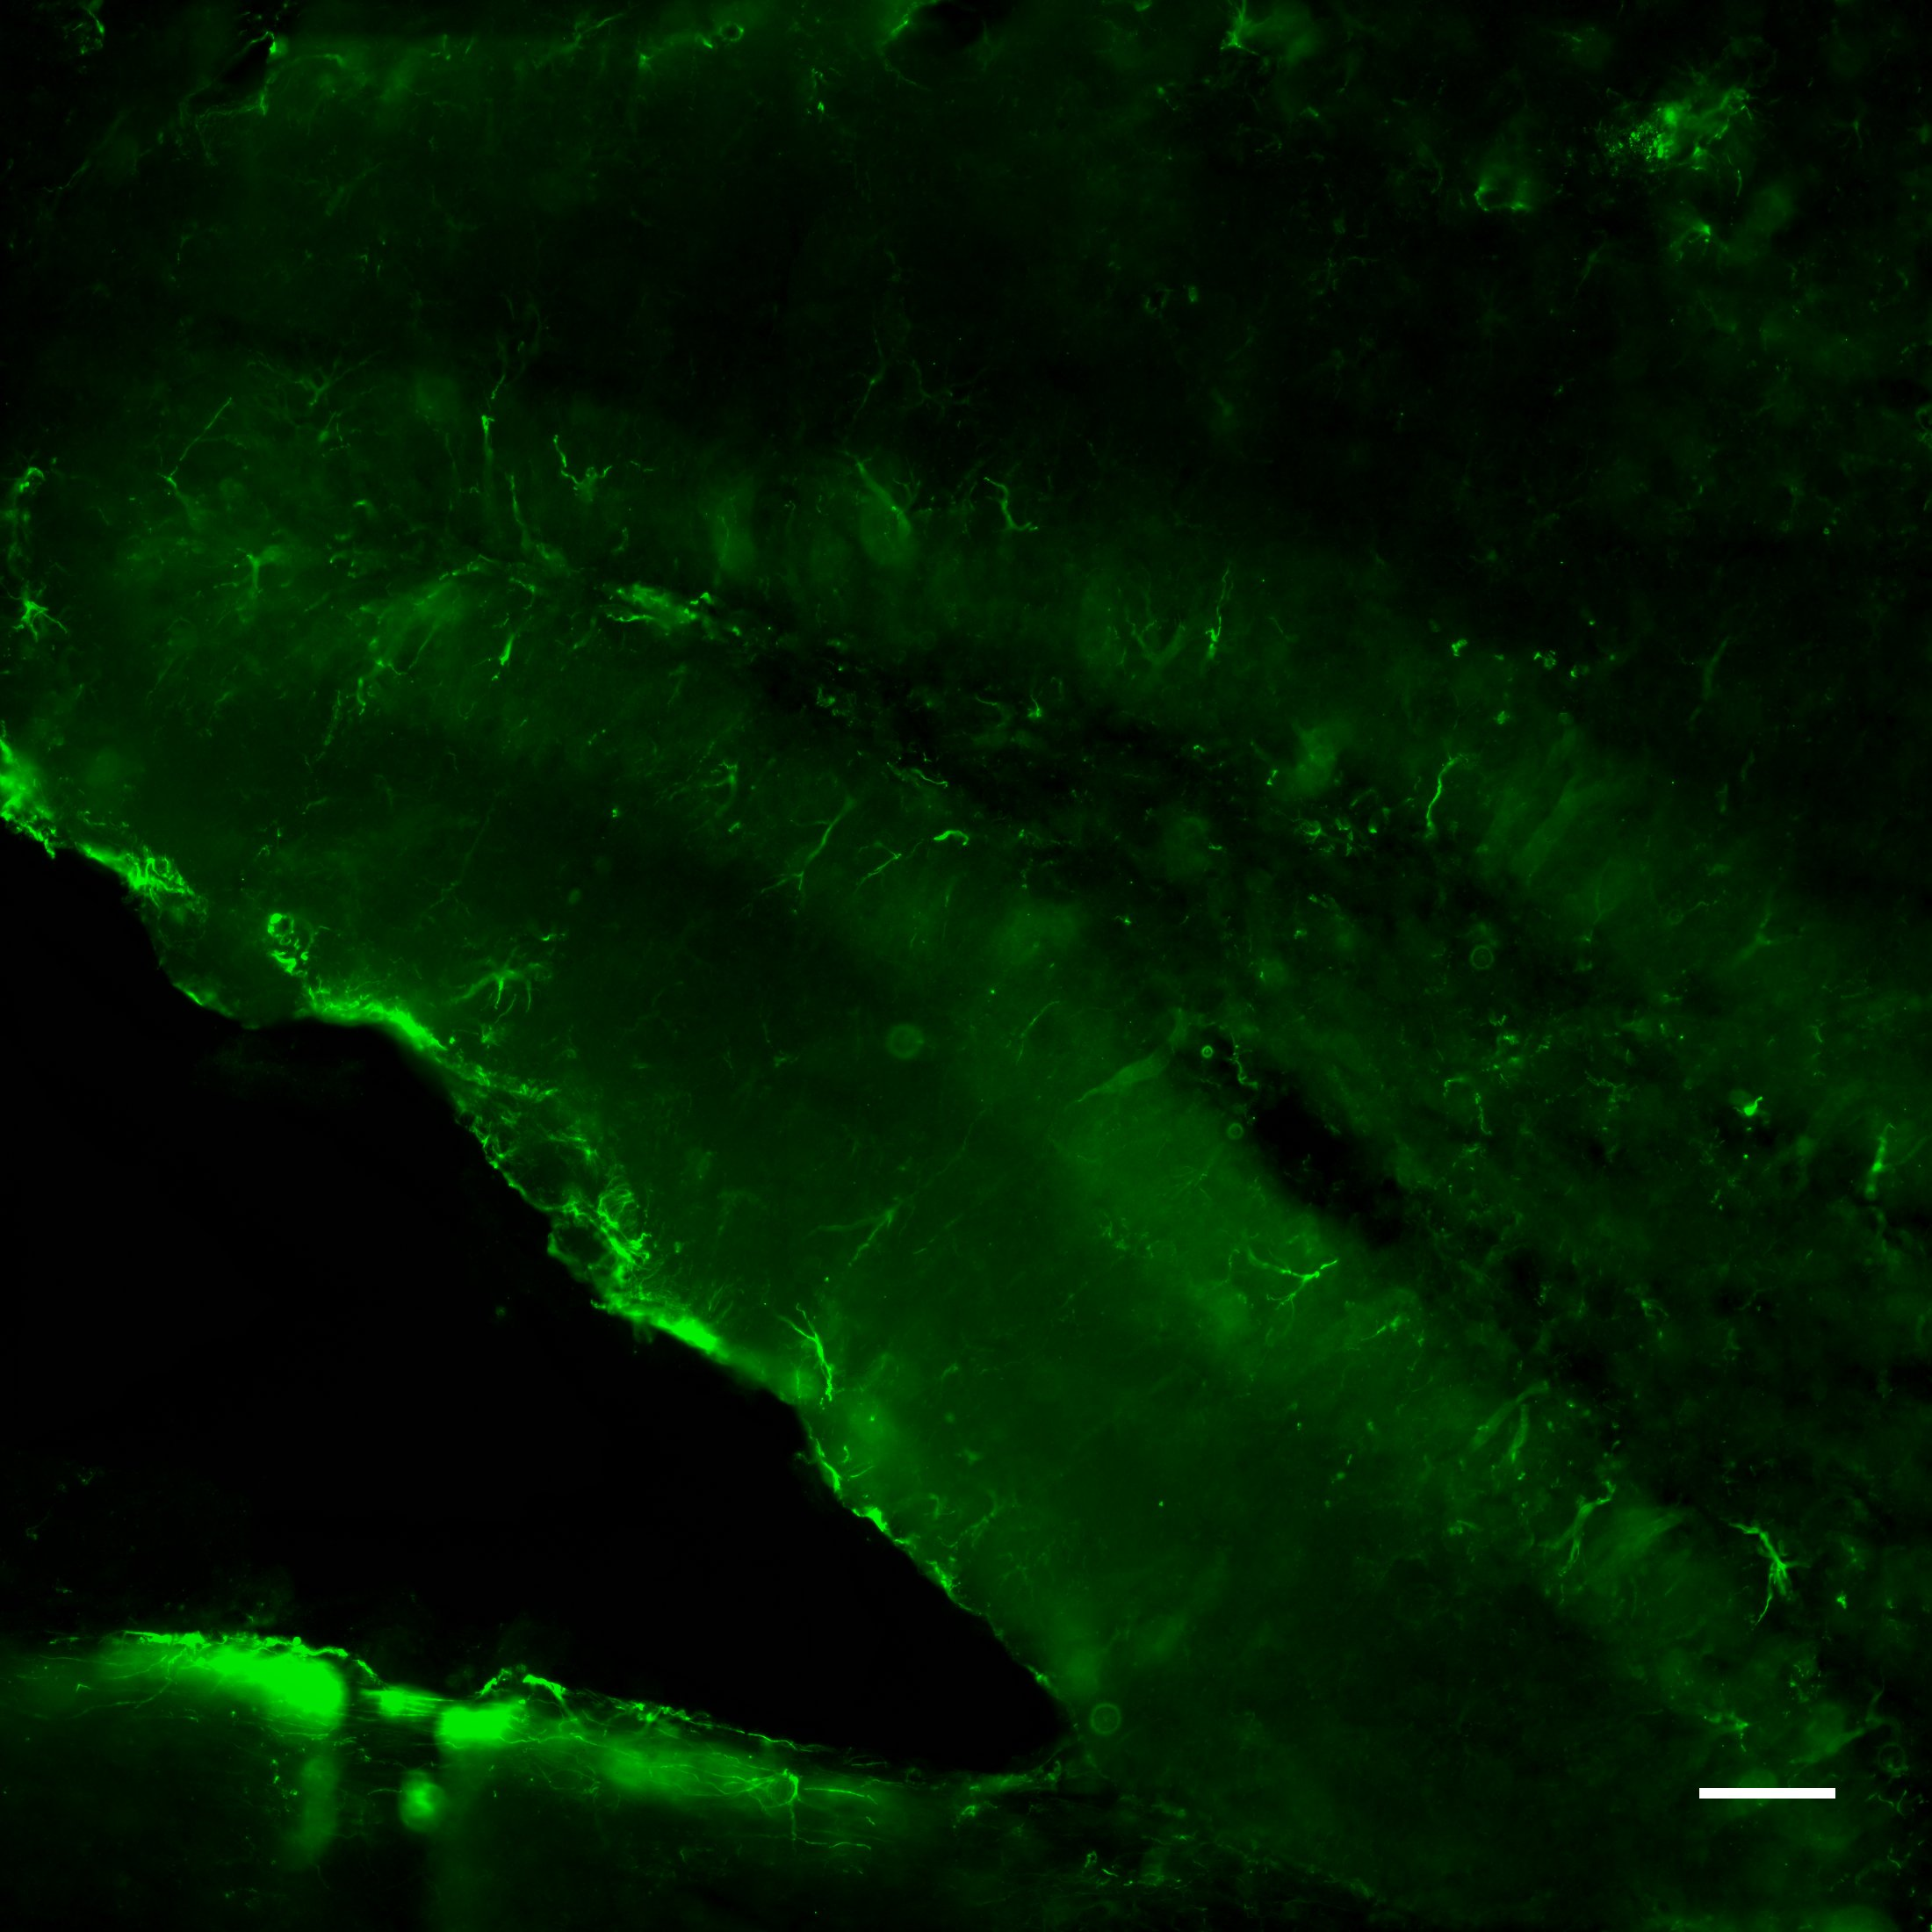
\includegraphics[width=\textwidth]{./Images/Immuno/Musk/MuSK_dg_50um.jpg}
		\end{subfigure}
		\begin{subfigure}[h]{0.245\textwidth}
			\caption{}
			\label{fig:locaMuSKhb}
			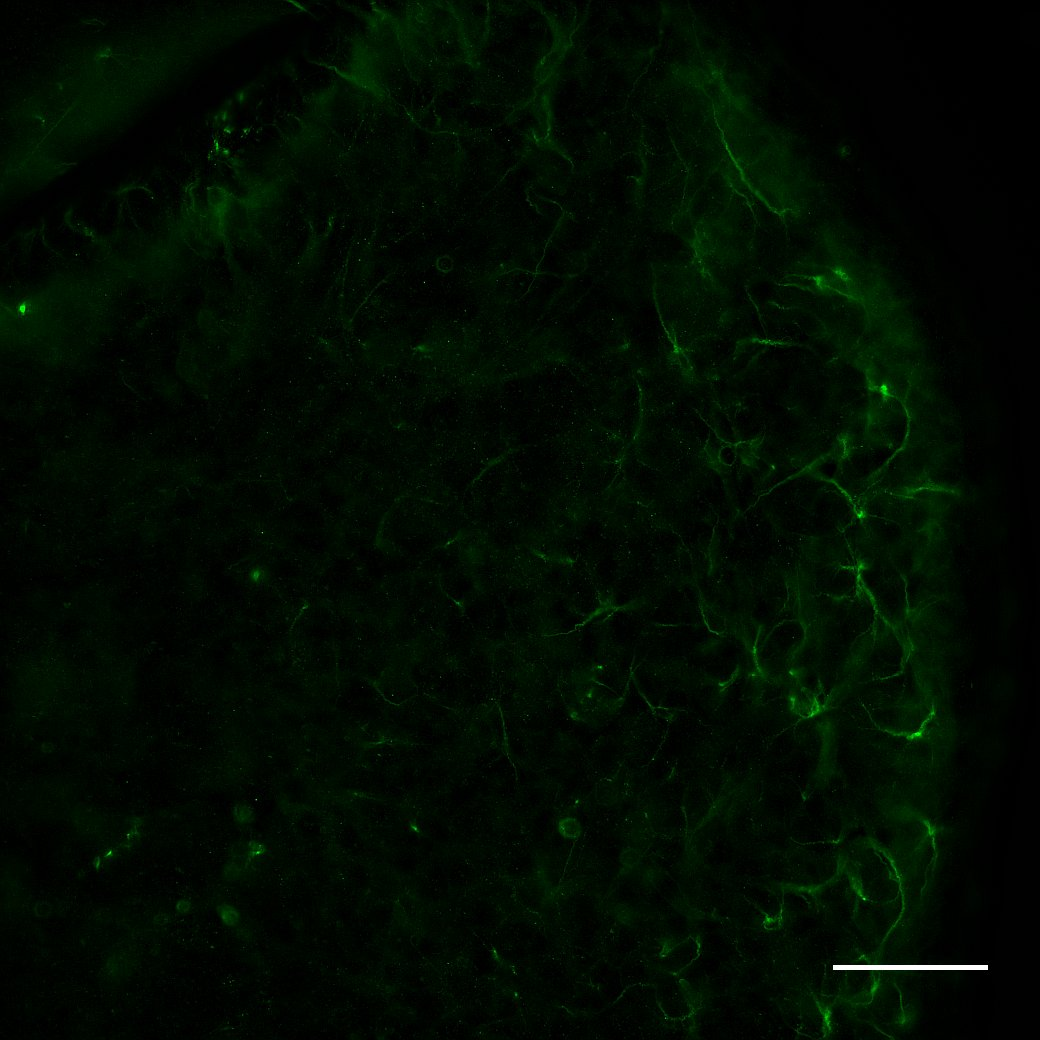
\includegraphics[width=\textwidth]{./Images/Immuno/Musk/MuSK_hb_50um.jpg}
		\end{subfigure}
		\begin{subfigure}[h]{0.245\textwidth}
			\caption{}
			\label{fig:locaMuSKfr}
			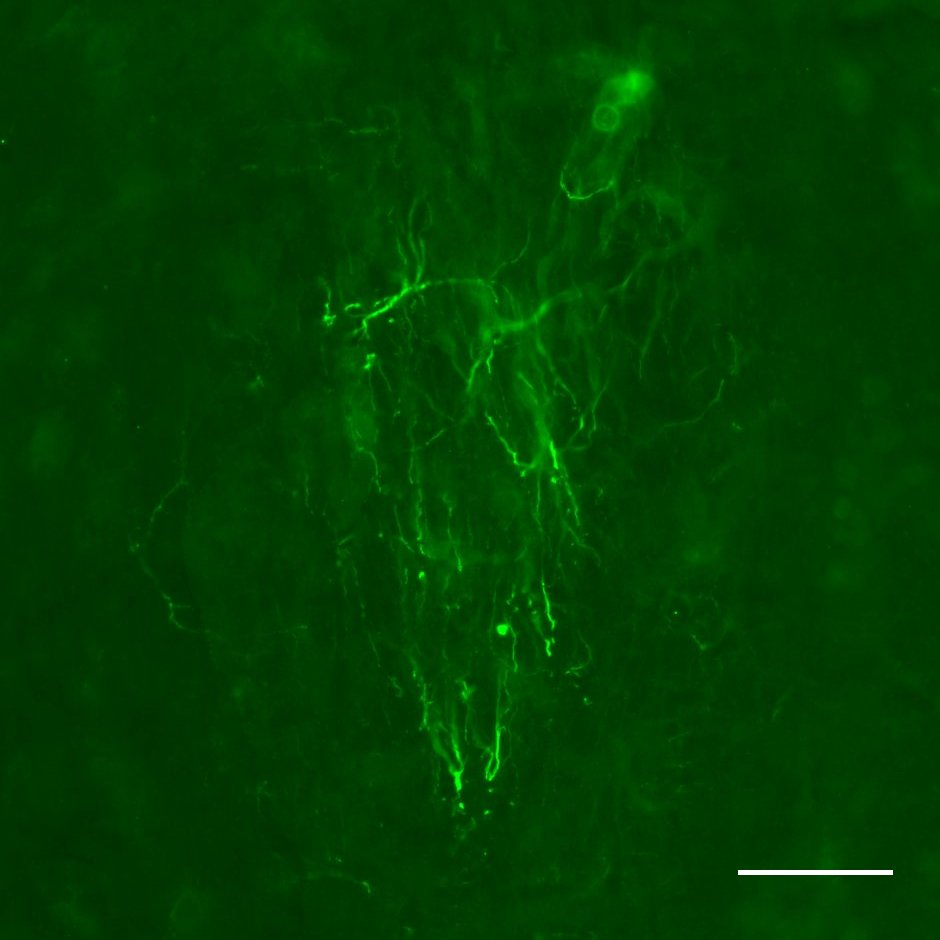
\includegraphics[width=\textwidth]{./Images/Immuno/Musk/MuSK_fr_50um.jpg}
		\end{subfigure}
		\begin{subfigure}[h]{0.395\textwidth}
			\caption{}
			\label{fig:locaMusKCtrl}
			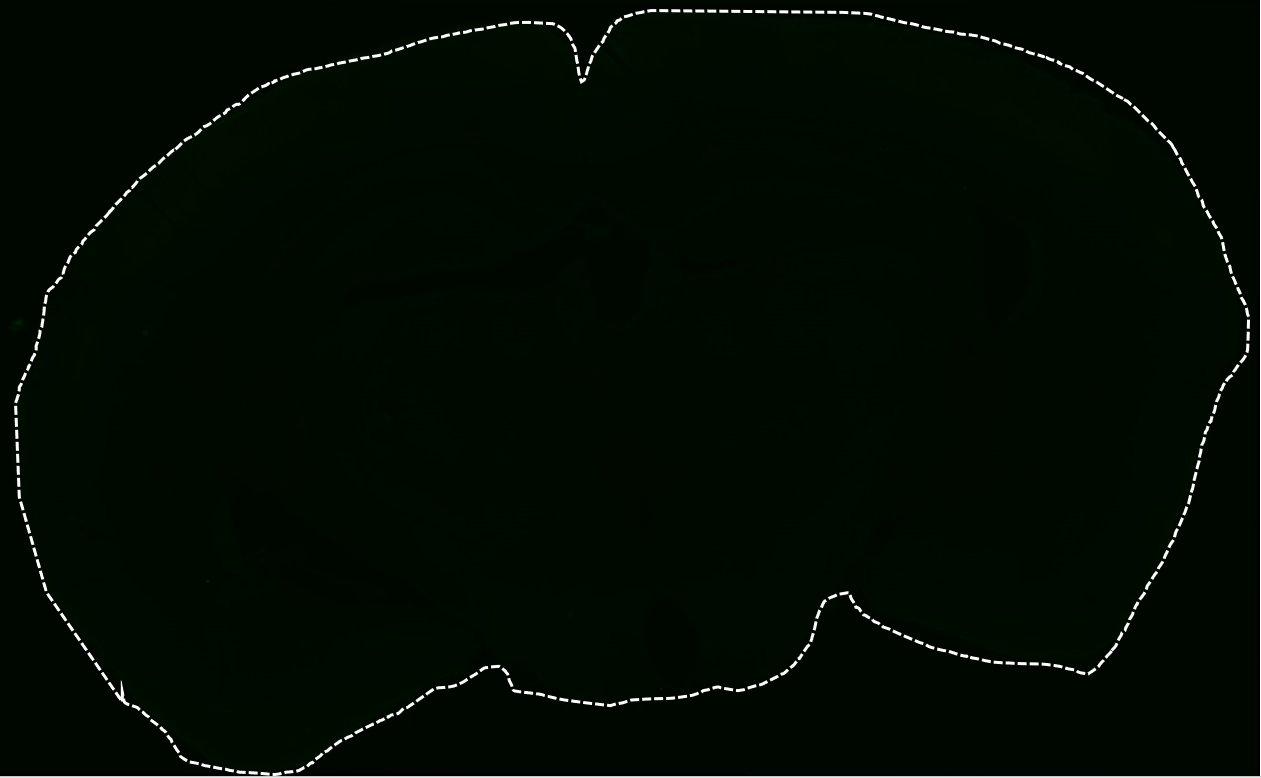
\includegraphics[width=\textwidth]{./Images/Immuno/Musk/loca_MuSK_ctrl.jpg}
		\end{subfigure}
		\caption{Localisation de \gls{musk} dans le cerveau.}
		\descfig{%
			\subref{fig:locaMusK} Immunomarquage de \gls{musk} sur coupe de cerveau entière. Coupe de souris mutante, mais le marquage est semblable chez les souris sauvages. %
			\subref{fig:locaMuSKcc} Zoom sur l'organisation du marquage au niveau du corps calleux. %
			\subref{fig:locaMuSKca1} Zoom sur l'organisation du marquage au niveau de la région CA1. L'épaississement vert correspond à la présence de noyau de la couche pyramidale. %
			\subref{fig:locaMuSKdg} Zoom sur l'organisation du marquage au niveau du Gyrus Denté. %
			\subref{fig:locaMuSKhb} Zoom sur l'organisation du marquage au niveau de l'habenula médiale. %
			\subref{fig:locaMuSKfr} Zoom sur l'organisation du marquage au niveau du fasciculus retroflexus. %
			\subref{fig:locaMusKCtrl} Coupe contrôle du marquage de \gls{musk}. Aucun marquage n'apparaît. %
			 alv : alveus hippocampus, cc : corps calleux, cp : pédoncule cérébral, ec : capsule externe, fr : fasciculus retroflexus, hp : hippocampe, or : stratum oriens de l'hippocampe. Barre d'échelle : 2 mm (\subref{fig:locaMusK}, \subref{fig:locaMusKCtrl}), 50µm (\subref{fig:locaMuSKcc}- \subref{fig:locaMuSKfr}).
			 	}
		\label{fig:ImmunoMusk}
	\end{figure}
	\FloatBarrier
	
	Dans ces régions, \gls{musk} est présent dans des prolongements cellulaires. La structure des cellules marquées par l'anticorps anti-\gls{musk} étant réminiscente de celles des astrocytes, un co-marquage de \gls{musk} et \gls{gfap}, une protéine spécifique du cytosquelette des astrocytes a été réalisé.
	
	Pour réaliser le marquage de \gls{gfap}, deux anticorps différents ont été utilisés. Le premier, fourni par l'équipe de C. AGULHON, provient de chez Millipore-Merck (\cref{table:Ac}, réf. MAB360) et a permis de visualiser des marquages spécifique. Le second anticorps, provenant de chez Abcam (\cref{table:Ac}, réf. ab4648) et commandé suite à une indisponibilité du premier anticorps, s'est révélé inefficace à différentes concentrations testées ($1{:}100$, $1{:}50$). Le premier anticorps a pu heureusement être à nouveau obtenu pour la suite des expériences.
	
	Suite au co-marquage de \gls{musk} et \gls{gfap}, on peut observer une colocalisation des deux marqueurs, ce qui semblerait indiqué que \gls{musk} est exprimé par les astrocytes (\cref{fig:ColocMuSK,fig:ColocGFAP,fig:ColocMuSK&GFAP}). 
	
	F. Semprez, un autre membre de l'équipe à montrer qu'en plus du cerveau, \gls{musk} est également présent dans la substance blanche de la moëlle épinière, et colocalise avec \gls{gfap} (\cref{fig:MuSKME}).
	
	%Images Coloc. MuSK GFAP
	\begin{figure}[h]
		\begin{subfigure}[h]{0.329\textwidth}
			\caption{}
			\label{fig:ColocMuSK}
			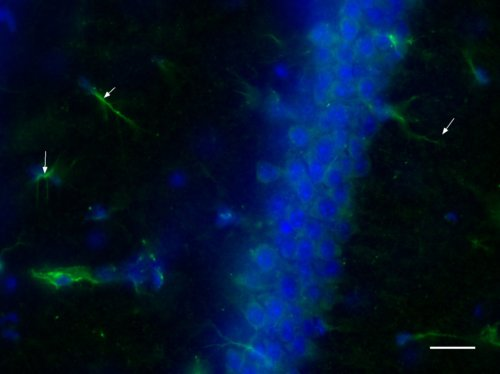
\includegraphics[width=\textwidth]{./Images/Immuno/Musk/MuSK-GFAP/M439_Mut_MuSK.jpg}
		\end{subfigure}
		\begin{subfigure}[h]{0.329\textwidth}
			\caption{}
			\label{fig:ColocGFAP}
			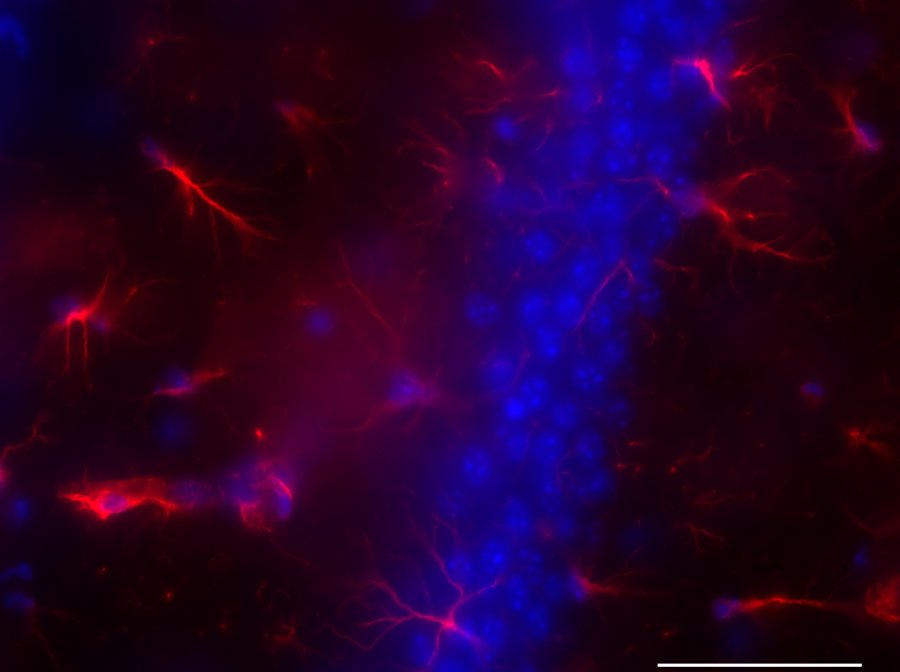
\includegraphics[width=\textwidth]{./Images/Immuno/Musk/MuSK-GFAP/M439_Mut_GFAP.jpg}
		\end{subfigure}
		\begin{subfigure}[h]{0.329\textwidth}
			\caption{}
			\label{fig:ColocMuSK&GFAP}
			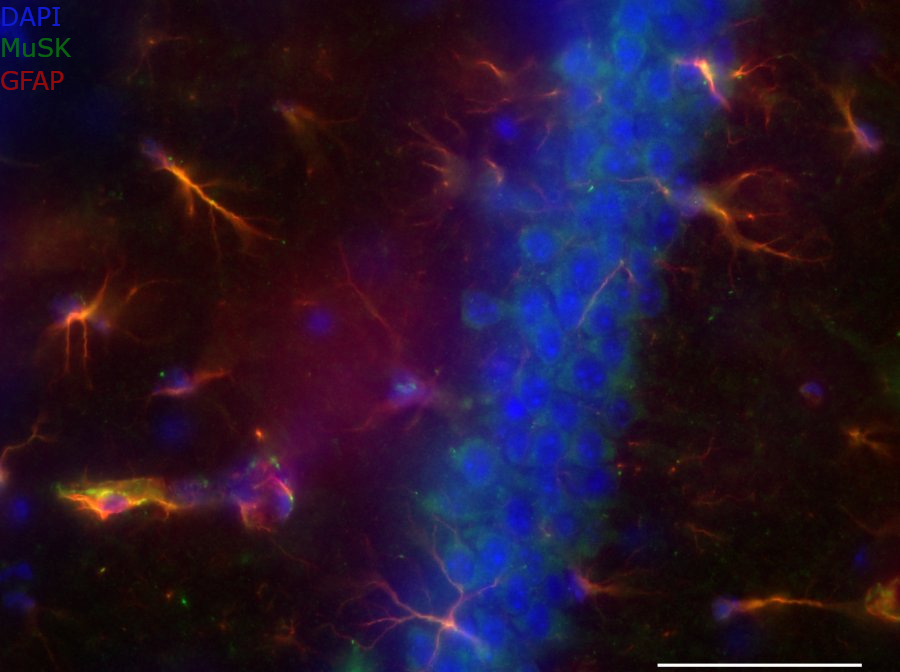
\includegraphics[width=\textwidth]{./Images/Immuno/Musk/MuSK-GFAP/M439_Mut_MuSK_GFAP.jpg}
		\end{subfigure}
		\begin{subfigure}[h]{0.329\textwidth}
			\caption{}
			\label{fig:ColocZoom}
			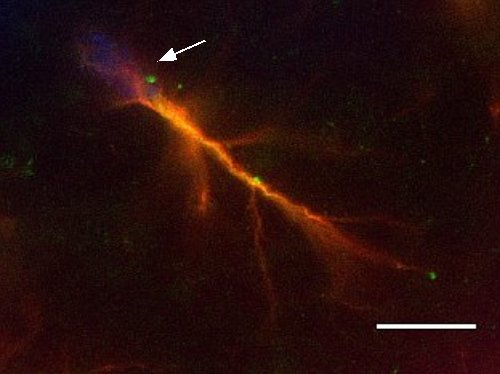
\includegraphics[width=\textwidth]{./Images/Immuno/Musk/MuSK-GFAP/zoom10um.jpg}
		\end{subfigure}
		\begin{subfigure}[h]{0.329\textwidth}
			\caption{}
			\label{fig:MuSKME}
			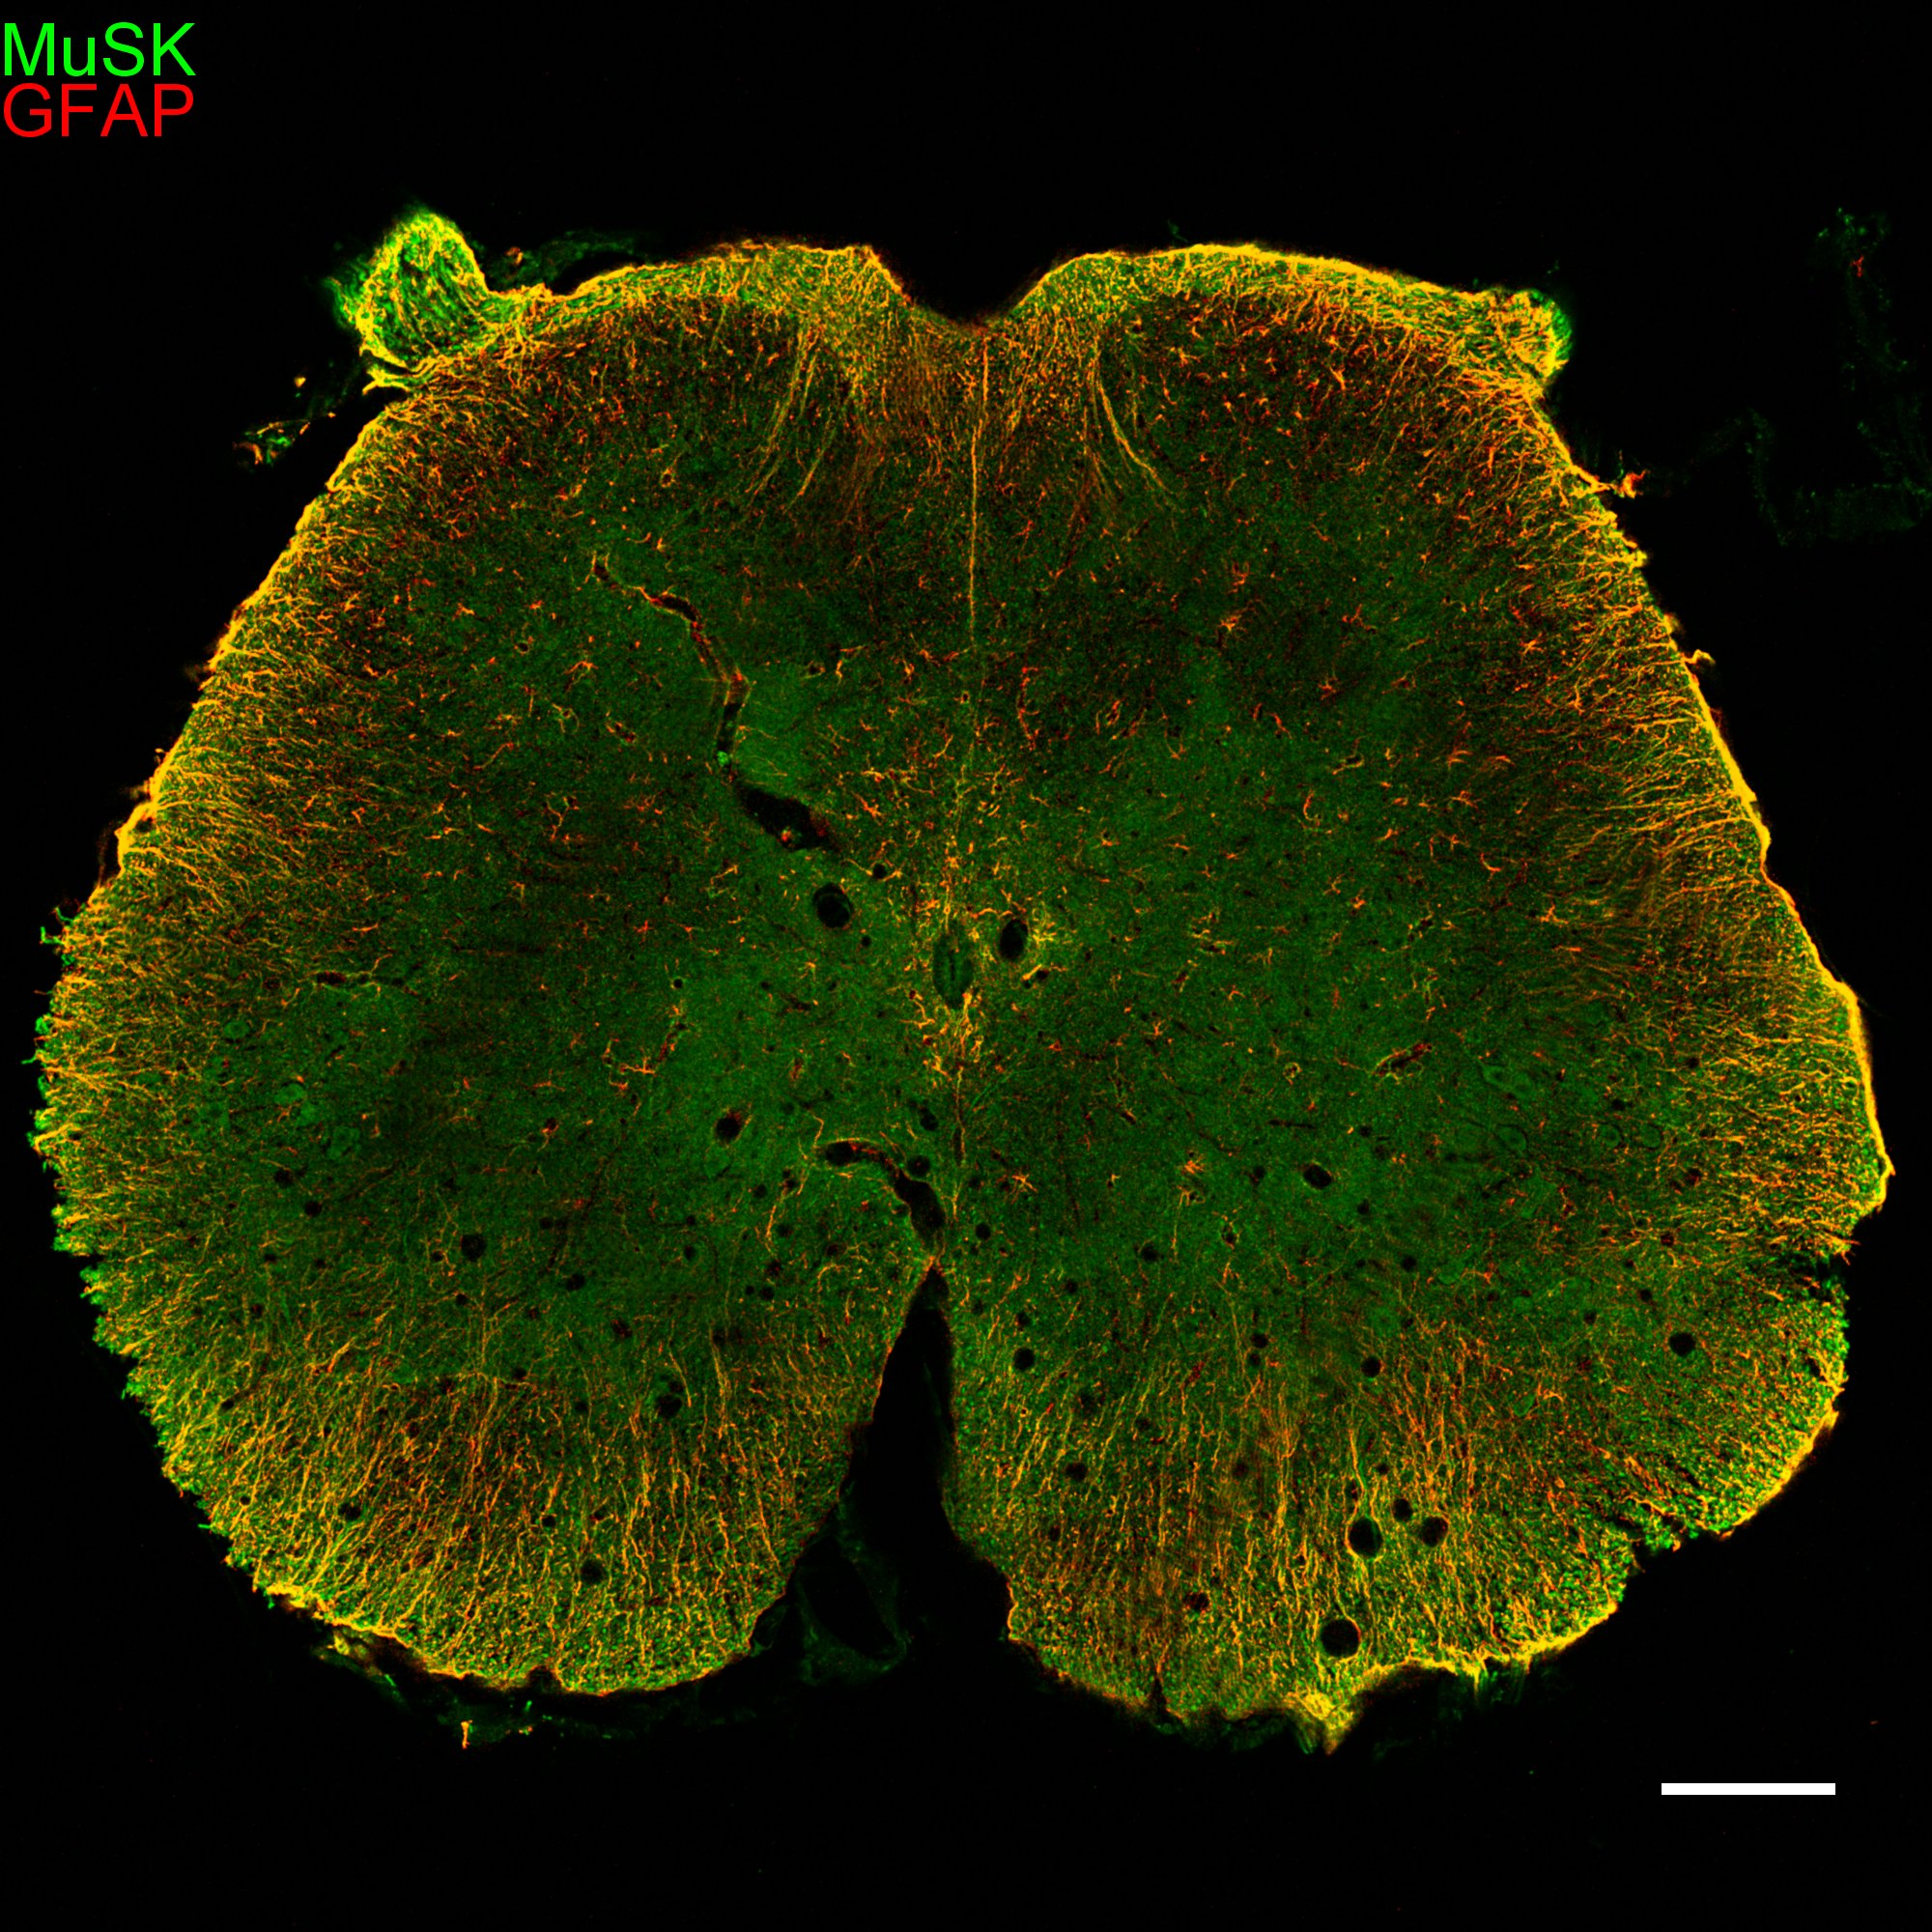
\includegraphics[width=\textwidth]{./Images/Immuno/Musk/Moelle_MuSK_GFAP_150um.jpg}
		\end{subfigure}
		\caption{Le marquage de \gls{musk} et \gls{gfap} colocalise.}
		\descfig{%
			Marquage de \gls{musk} (vert) et de \gls{gfap} (rouge) et \acrshort{dapi} (bleu) au niveau de la région CA1 de l'hippocampe. Le marquage de \gls{musk} va colocaliser avec \gls{gfap} dans toutes les régions du cerveau observées.
			\subref{fig:ColocMuSK} Marquage de \gls{musk}.
			\subref{fig:ColocGFAP} Marquage de \gls{gfap}.
			\subref{fig:ColocMuSK&GFAP} Superposition de \subref{fig:ColocMuSK} et \subref{fig:ColocGFAP}.
			\subref{fig:ColocZoom} Zoom de la partie encadré de \subref{fig:ColocMuSK&GFAP}. On peut observer que le prolongement marqué à la fois par \gls{musk} et \gls{gfap} va se mettre en place autour du noyau (flèche blanche).
			\subref{fig:MuSKME} Co-marquage de \gls{musk} et de \gls{gfap} au niveau de la moëlle épinière.
			Barre d'échelle : 150µm \subref{fig:MuSKME} ; 20µm \subref{fig:ColocMuSK}, \subref{fig:ColocGFAP}, \subref{fig:ColocMuSK&GFAP} ; 10µm \subref{fig:ColocZoom}.
				}	
		\label{fig:colocalisation}
	\end{figure}
\FloatBarrier
	
	Cependant, le marquage observé de \gls{musk} ne ressemble pas à ce que l'on peut observer au niveau de la \gls{jnm}.  On peut donc émettre un doute sur la spécificité du marquage. Comme il n'existe pas vraiment d'autres anticorps dirigés contre \gls{musk} utilisables en \gls{ihc}, j'ai dû essayé d'autres moyen afin de tenter de confirmer la spécificité du marquage. Tout d'abord, un co-marquage \gls{musk}/\acrshort{gfap} à été réalisé sur des sections de cerveau d'embryon de souris \gls{musk} KO (stade E18.5), la mutation étant létale après la naissance pour cause de défaillance respiratoire (\cref{fig:MuskEmbryon}). Sur seulement une coupe d'embryon WT sur cinq, un léger marquage ressemblant à celui observer chez les adultes est présent (\cref{fig:MuskE5WT,fig:MuskE5Marquage}), et aucun marquage n'est présent chez les animaux KO (\cref{fig:MuskE1KO}). Cela ne suffit pas à confirmer la spécificité du marquage de \gls{musk}. Pour tenter alors de confirmer la présence de \gls{musk} dans le cerveau, une immunoprécipitation est alors envisagée.
	
	%Images Embryon
	\begin{figure}[h]
		\begin{center}
			\begin{subfigure}[h]{0.329\textwidth}
				\caption{}
				\label{fig:MuskE5WT}
				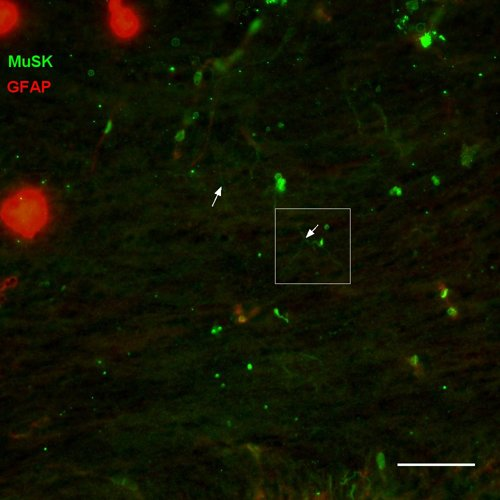
\includegraphics[width=\textwidth]{./Images/Immuno/Musk/Embryon/E5WT_50um_500px_df.jpg} 
			\end{subfigure}
			\begin{subfigure}[h]{0.329\textwidth}
				\caption{}
				\label{fig:MuskE5Marquage}
				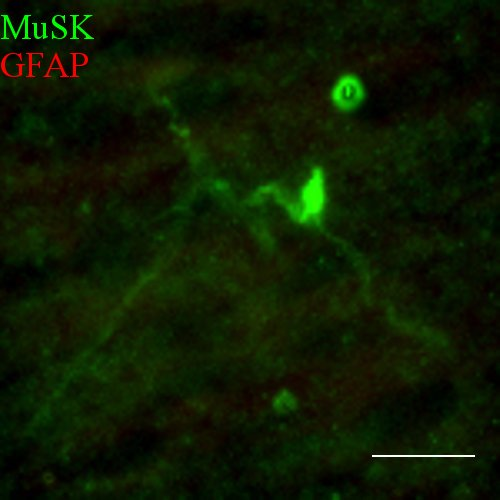
\includegraphics[width=\textwidth]{./Images/Immuno/Musk/Embryon/E5_WT_MuSK_500px_Zoom_10um.jpg}
			\end{subfigure}
			\begin{subfigure}[h]{0.329\textwidth}
				\caption{}
				\label{fig:MuskE1KO}
				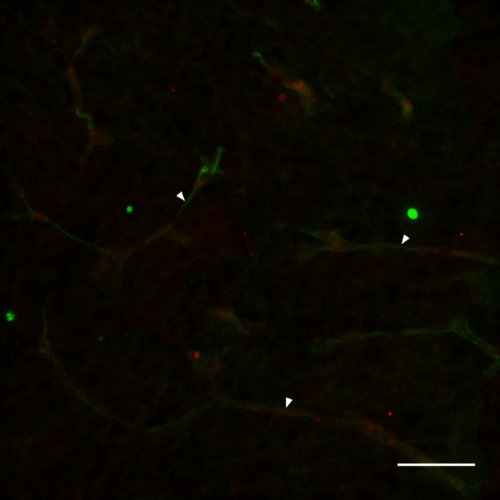
\includegraphics[width=\textwidth]{./Images/Immuno/Musk/Embryon/E1KO_50um_500px_df.jpg}
			\end{subfigure}
		\end{center}
		\caption{Pas de marquage de \gls{musk} sur embryon E18.5 WT et KO.}
		\descfig{%
			Marquage de \gls{musk} et \gls{gfap} sur des embryons (stade E18.5) de souris \gls{musk} KO (n = 2) et WT (n = 1). %
			\subref{fig:MuskE5WT} Embryon WT. Sur une coupe, un marquage ressemblant à celui de \gls{musk} observé chez les adultes était présent (flèches blanches). %
			\subref{fig:MuskE5Marquage} Agrandissement du marquage de \gls{musk} encadré en \subref{fig:MuskE5WT}. %
			\subref{fig:MuskE1KO} Embryon KO. Le marquage observé (triangles blanc) n'est pas spécifique. %
			Images représentatives issues de la région du fornix dorsal. Barre d'échelle : 50µm \subref{fig:MuskE5WT} et  \subref{fig:MuskE1KO}, 10µm \subref{fig:MuskE5Marquage}. 
				}
		\label{fig:MuskEmbryon}
	\end{figure}
\FloatBarrier

	Afin d'identifier plus précisément le ou les types de cellules exprimant \gls{musk}, un co-marquage entre le récepteur et différents marqueurs a été réalisé sur des cultures primaires d'hippocampes, cultures issues d'embryon au stade E16 puis cultivées 14 jours, fourni par D. Carrel. Les marqueurs cellulaires sont \gls{gfap} pour marquer les astrocytes et \gls{map2} pour marquer les dendrites des neurones. J'ai également testé un co-marquage \gls{musk} et \gls{glt1}, marqueur membranaire astrocytaire d'un transporteur du glutamate, afin de voir si \gls{musk} était localisé à la membrane, mais ce marquage n'a pas fonctionné.
	
	\todo{a reformuler}
	Les co-marquages de cultures cellulaires ont permis de confirmer la localisation observée sur les coupes de cerveaux de \gls{musk}, qui est présent dans les prolongements astrocytaires (\cref{fig:CultureMGgfapmusk}). On observe également sur les images des prolongements cellulaires marqués par \gls{musk} qui ne sont pas co-marqués avec la \gls{gfap}.
	
	\gls{map2} est un marqueur des dendrites des neurones. Lors du co-marquage avec \gls{musk}, on peut voir sur les cultures certains prolongements sont à la fois marqués par \gls{map2} et par \gls{musk} (\cref{fig:CultureMMmap2}). Les prolongements non marqués ont une morphologie semblable à ceux marqués par \gls{gfap} : il s'agit ainsi du marquage d'astrocytes. En plus du marquage de prolongements, \gls{map2} va aussi être localisé dans le cytoplasme, autour de noyaux (\cref{fig:CultureMMmap2musk}, flèches blanches) qui va aussi co-localisé avec \gls{musk}. 
	
	La marquage de cultures cellulaires montre ainsi que non seulement \gls{musk} va être exprimé par les astrocytes, dans les prolongement mais aussi dans le corps cellulaire, comme observé sur les coupes de cerveaux, mais que le récepteur est aussi présent dans les neurones. \Gls{musk} est observé dans les dendrites, mais également dans le cytoplasme des cellules, chose qui n'était pas visible précédemment.
		
	%Images cultures cellulaire
	\clearpage	
	\begin{figure}
		\begin{subfigure}[h]{0.329\textwidth}
			\caption{}
			\label{fig:CultureMGmusk}
			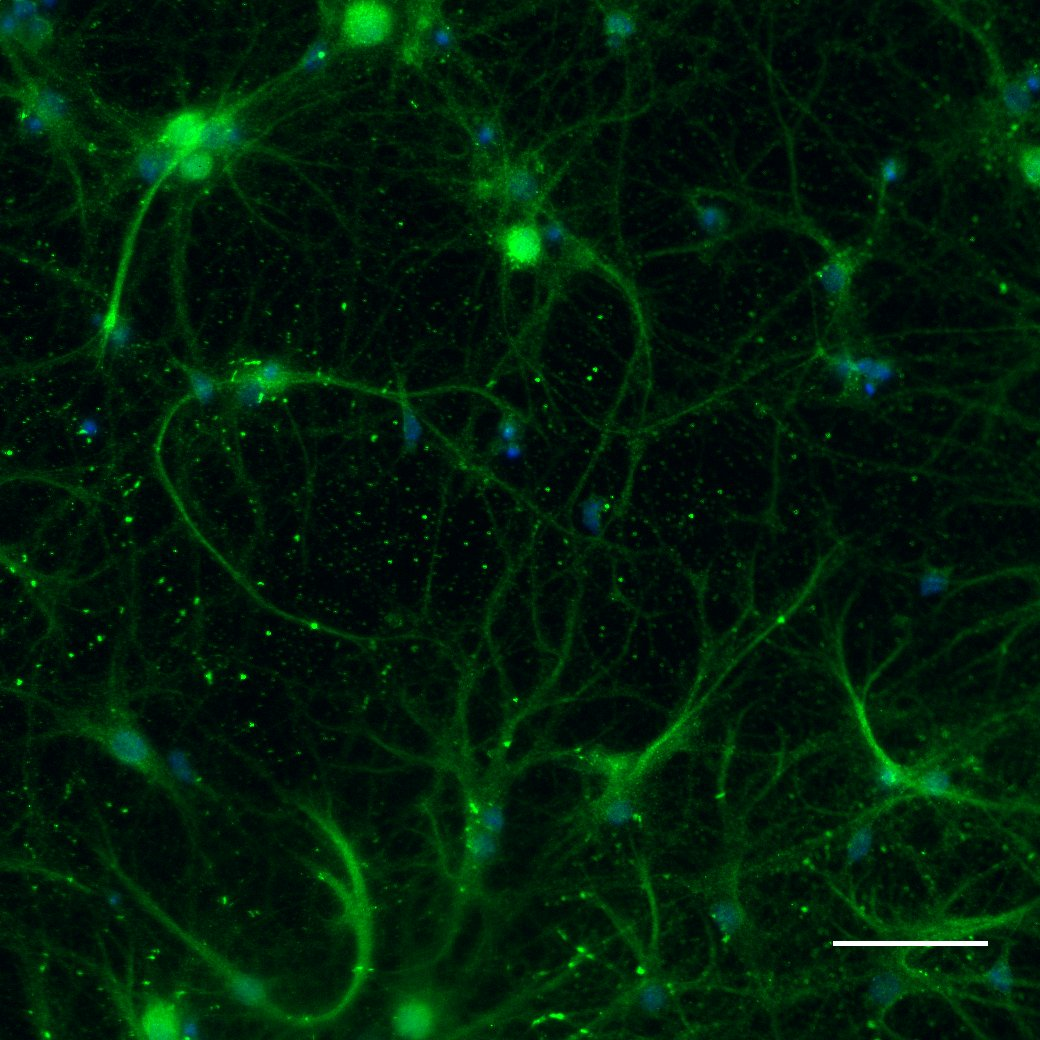
\includegraphics[width=\textwidth]{./Images/Immuno/Musk/Cultures/MuSK_50um.jpg}
		\end{subfigure}
		\begin{subfigure}[h]{0.329\textwidth}
			\caption{}
			\label{fig:CultureMGgfap}
			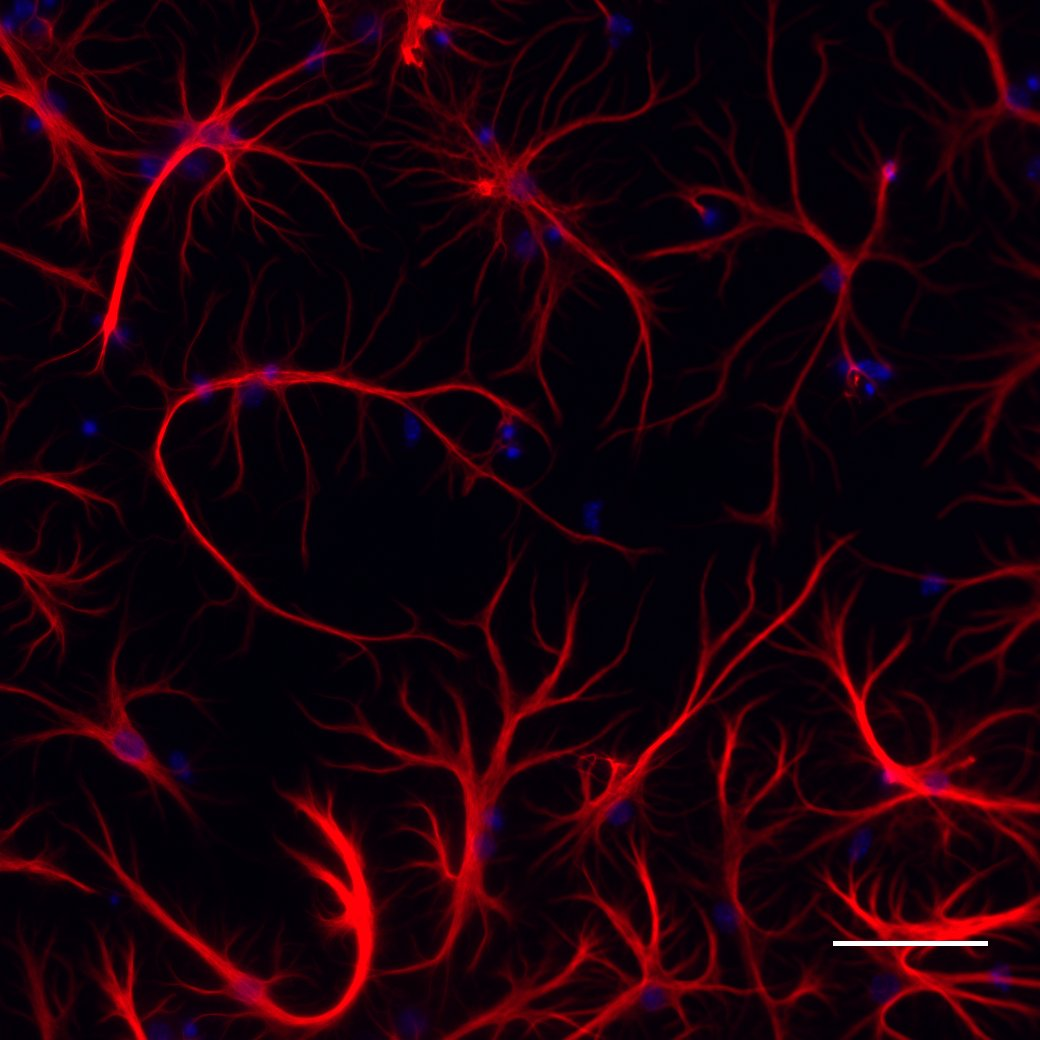
\includegraphics[width=\textwidth]{./Images/Immuno/Musk/Cultures/GFAP_50um.jpg}
		\end{subfigure}
		\begin{subfigure}[h]{0.329\textwidth}
			\caption{}
			\label{fig:CultureMGgfapmusk}
			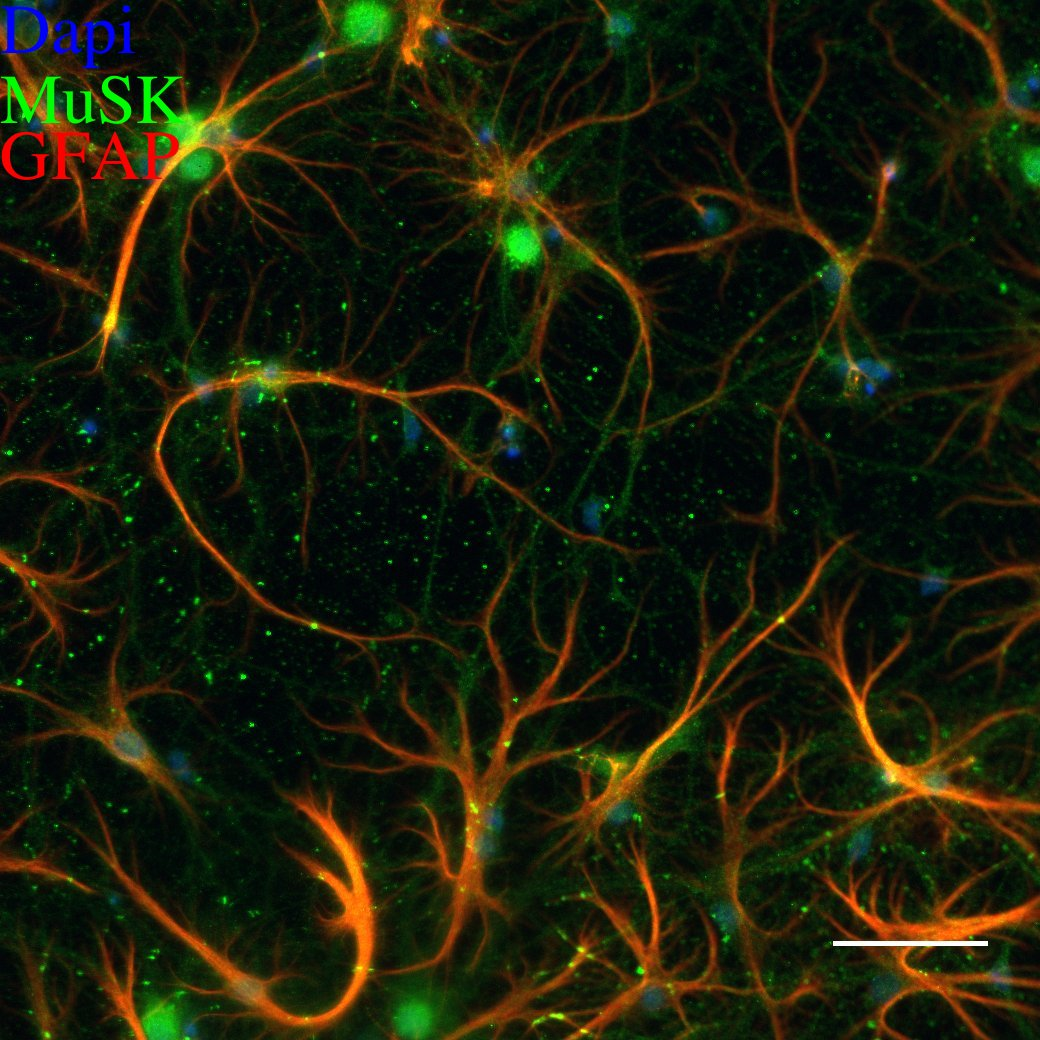
\includegraphics[width=\textwidth]{./Images/Immuno/Musk/Cultures/GFAP-MuSK_50um.jpg}
		\end{subfigure}
		\begin{subfigure}[h]{0.329\textwidth}
			\caption{}
			\label{fig:CultureMMmusk}
			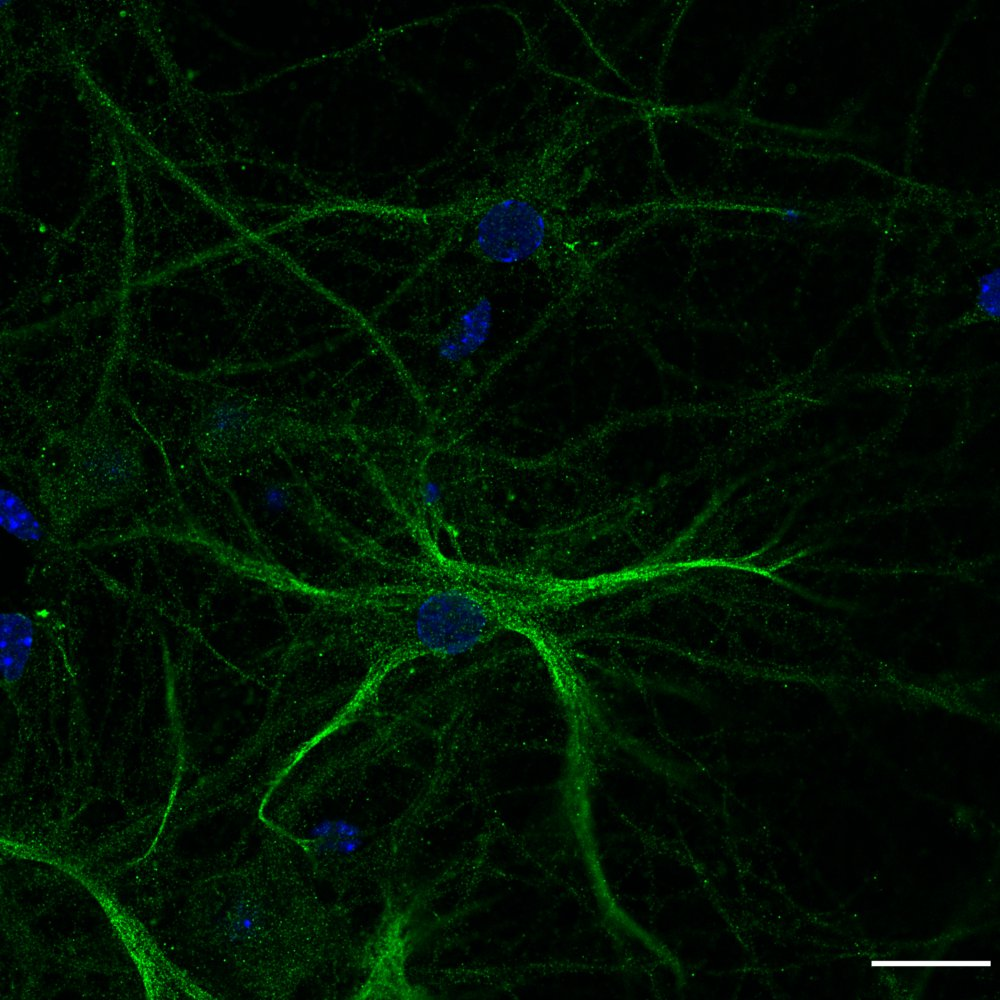
\includegraphics[width=\textwidth]{./Images/Immuno/Musk/Cultures/MuSK_20um.jpg}
		\end{subfigure}
		\begin{subfigure}[h]{0.329\textwidth}
			\caption{}
			\label{fig:CultureMMmap2}
			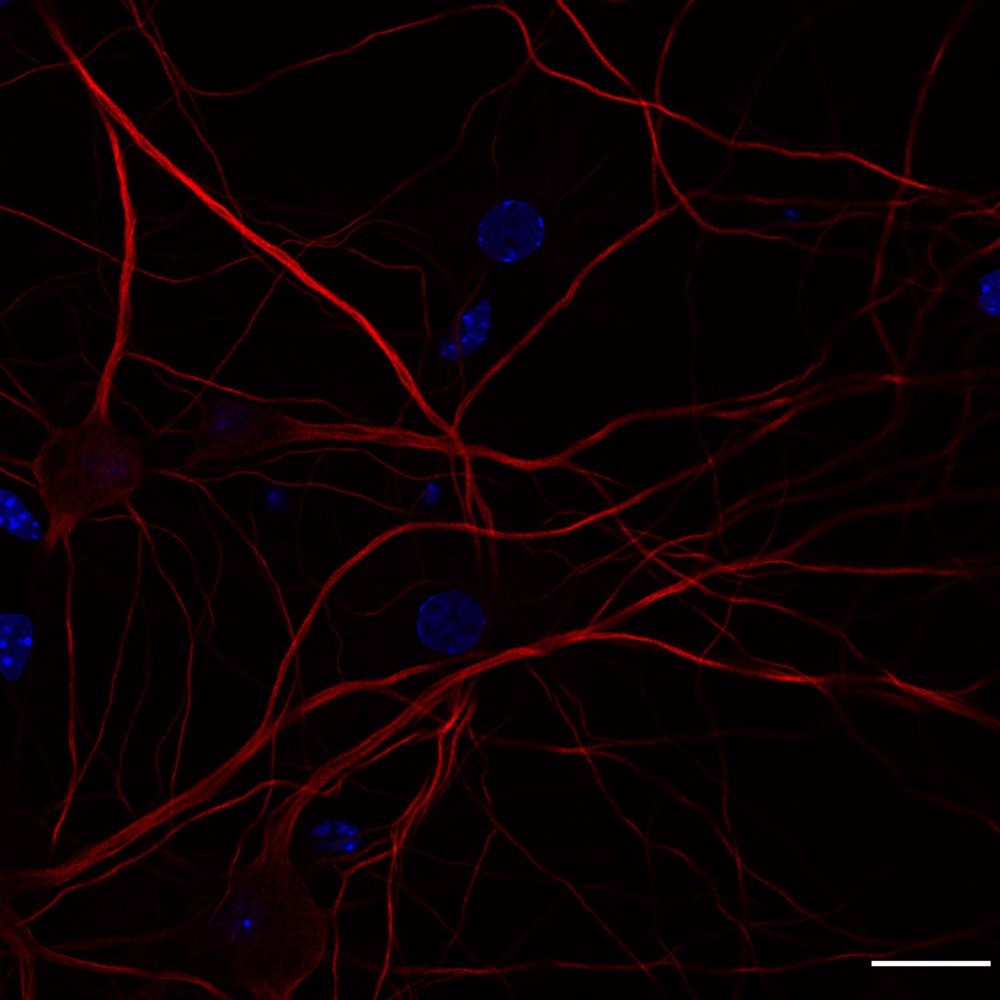
\includegraphics[width=\textwidth]{./Images/Immuno/Musk/Cultures/MAP2_20um.jpg}
		\end{subfigure}
		\begin{subfigure}[h]{0.329\textwidth}
			\caption{}
			\label{fig:CultureMMmap2musk}
			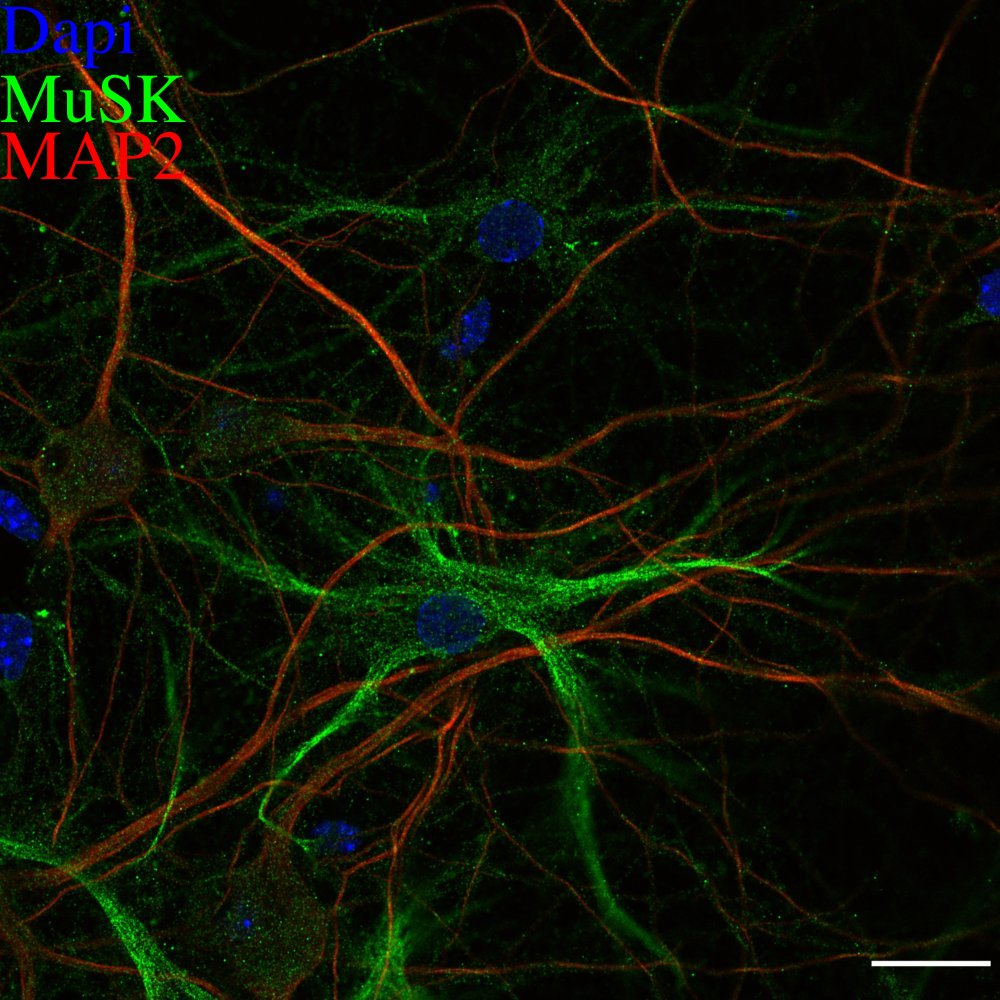
\includegraphics[width=\textwidth]{./Images/Immuno/Musk/Cultures/MuSK-MAP2_20um.jpg}
		\end{subfigure}
	\caption{Co-marquage de \gls{musk} et \gls{gfap} (astrocytes) et \gls{map2} (neurones) sur une culture d'hippocampe.}
	\descfig{%
					Co-marquage de \gls{musk} (vert), \acrshort{dapi} (bleu) et \gls{map2} (rouge, \subref{fig:CultureMMmusk}-\subref{fig:CultureMMmap2musk}) et \gls{gfap} (rouge, \subref{fig:CultureMGmusk}-\subref{fig:CultureMGgfapmusk}).
					\subref{fig:CultureMGmusk} Marquage de \gls{musk}
					\subref{fig:CultureMGgfap} Marquage de \gls{gfap}
					\subref{fig:CultureMGgfapmusk} Merge 
					\subref{fig:CultureMMmusk} Marquage de \gls{musk}
					\subref{fig:CultureMMmap2} Marquage de \gls{map2}
					\subref{fig:CultureMMmap2musk} Merge. Flèches blanches : marquage cytoplasmique de \gls{map2} et de \gls{musk}.
					Barre d'échelle : 20µm (\subref{fig:CultureMMmusk}-\subref{fig:CultureMMmap2musk}), 50µm (\subref{fig:CultureMGmusk}-\subref{fig:CultureMGgfapmusk}).
					}
	\label{fig:MuSKMAP2GFAP}
	\end{figure}
	\FloatBarrier

\section{Immunoprécipitation}
\label{sec:IPresultat}
	Afin de confirmer la détection de \gls{musk} dans diverse région du cerveau, une immunoprécipitation suivie d'un \gls{wb} a été réalisée sur trois structures : l'hippocampe, le cervelet et le cortex de trois souris C57Bl/6 sauvage. Un \gls{wb} de \gls{musk} a déjà été décrit sur des diverses structures du cerveau \cite{Garcia-Osta2006}, mais à partir d'extrait total de protéines et non d'une \gls{ip}. Durant son stage, B. SOMON a tenté de réaliser un \gls{ip} suivi d'un \gls{wb}, mais sans obtenir de résultats probant. Ici, la principale modification apportée au protocole précédemment utilisée par cette étudiante est l'utilisation de tampon RIPA (adjonction de déoxycholate de sodium et de \acrshort{sds} dans le tampon) qui permet une meilleure lyse et une meilleure préservation des protéines lors de l'extraction.
	
	Afin de vérifier si la technique fonctionnait, j'ai tout d'abord prélevé l'hippocampe, le cervelet et le cortex de trois souris C57Bl/6 puis réalisé une \gls{ip} de \gls{musk} dessus, qui a ensuite été migré dans un gel pour un \gls{wb}. tout d'abord, comme l'anticorps utilisé pour l'\gls{ip} et la révélation était le même, un nouvel anticorps secondaire ciblant uniquement les chaines légères a été utilisé, afin d'éviter d'avoir trop de marquage non spécifique. Cependant, rien ne fut révélé, même le témoin positif était très faible, malgré un temps d'exposition important (supérieur à 30 minutes) (\cref{fig:WB-anti-LC}). La membrane à été deshybridées puis ré-incubée avec de l'anti-\gls{musk} ainsi qu'un autre anticorps secondaire dirigé contre les \glspl{ig} de lapin, qui à pour défaut d'être plus bruité (bande à 75kDa correspondant aux anticorps non couplés lors de l'\gls{ip}). Surprenamment, des bandes de taille attendue (110kDa) ont été révélée dans l'hippocampe et le cervelet (\cref{fig:WBbon}, flèches noires), alors que dans le cortex une bande d'intensité plus faible semblait être présente (\cref{fig:WBbon}, tête de flèche noire), ce qui pourrait correspondre au fait qu'il n'y ait pas dans cette région du cerveau de marquage de \gls{musk} par \gls{ihc}. 
	
	Comme la taille des bandes ne correspondaient pas tout à fait à celle du témoin positif (extrait de cellules transfectées HEK293, à 130kDa, \cref{fig:WBbon}, flèche blanche), l'expérience à été refaite avec des souris \mcrd et sauvages, issues de la même lignée. En effet, suite à la mutation, la protéine \gls{musk} à un poids moléculaire de ~80kDa : si c'est bien \gls{musk} qui est détécté, on devrait alors avoir un décalage entre les individus. Cette fois-ci cependant, l'expérience ne s'est pas montrée concluante, rien n'a été révélé (\cref{fig:WB1erechec}). Afin de confirmer ce résultat, l'expérience a finalement été tentée une troisième fois avec comme témoin positif les extraits protéiques de la première expérience (cervelet et cortex, plus assez d'extraits d'hippocampe pour recommencer). Cette fois encore, rien n'a été révélé (\cref{fig:WBpasbon}).
	
	%Western Blot	
	\begin{figure}[h]
		\begin{center}
			\begin{subfigure}[h]{0.49\textwidth}
				\caption{}
				\label{fig:WB-anti-LC}
				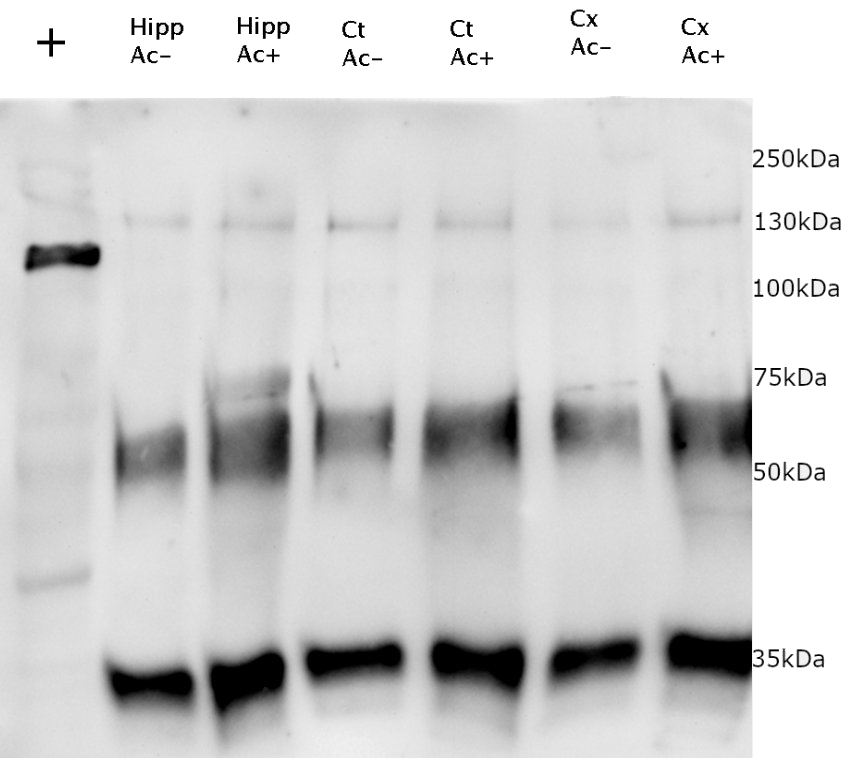
\includegraphics[width=\textwidth]{./Images/WB/@LC_MuSK_30'.jpg} %Gel anti light chain
			\end{subfigure}
			\begin{subfigure}[h]{0.49\textwidth}
				\caption{}
				\label{fig:WBbon}
				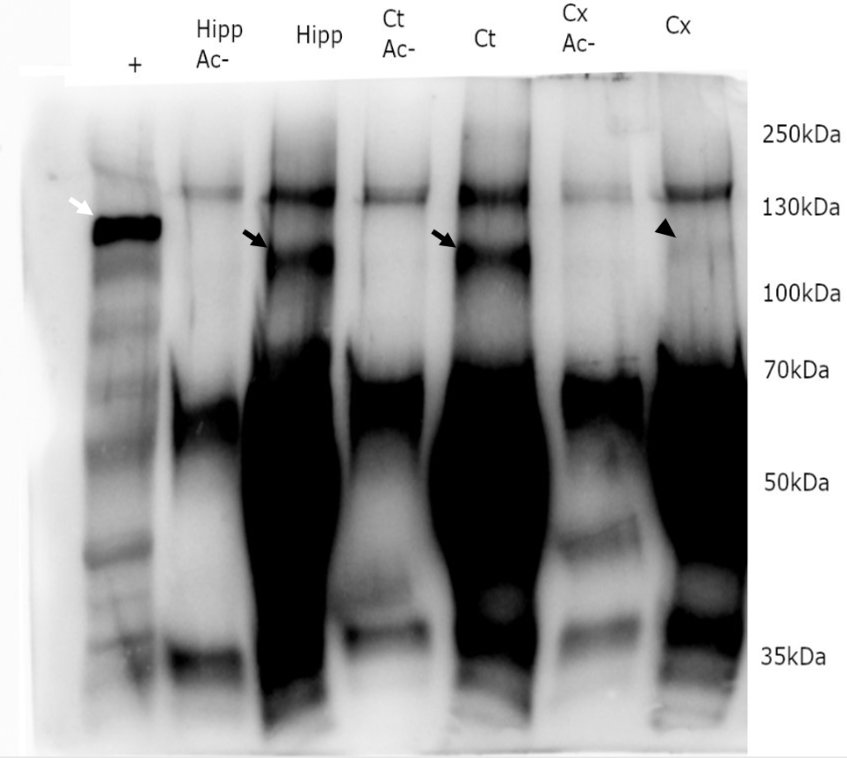
\includegraphics[width=\textwidth]{./Images/WB/2018-04-09.jpg} %Gel Bon :)
			\end{subfigure}
			\begin{subfigure}[h]{0.49\textwidth}
				\caption{}
				\label{fig:WB1erechec}
				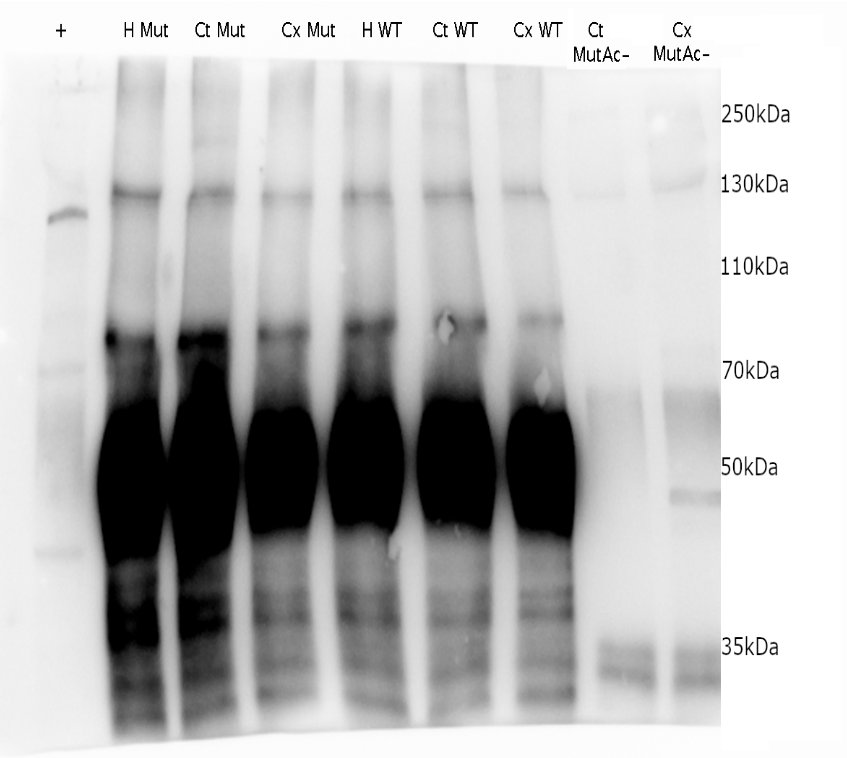
\includegraphics[width=\textwidth]{./Images/WB/2018-04-19.jpg} %Gel pas bon :(
			\end{subfigure}
			\begin{subfigure}[h]{0.49\textwidth}
				\caption{}
				\label{fig:WBpasbon}
				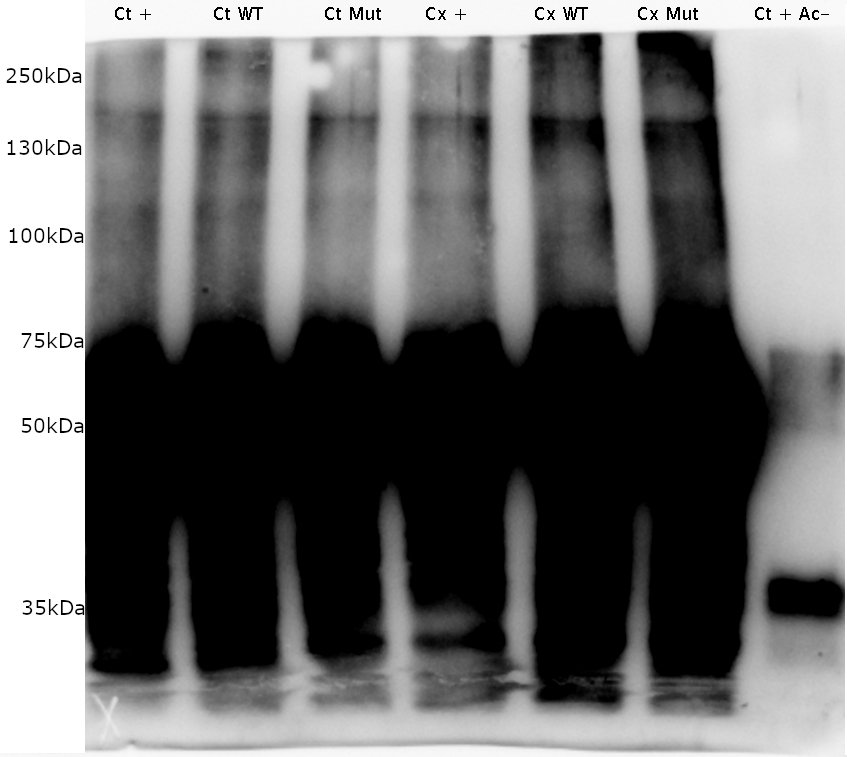
\includegraphics[width=\textwidth]{./Images/WB/2018-05-03.jpg} %Gel pas bon :(
			\end{subfigure}
		\end{center}
		\caption{L'\gls{ip} de \gls{musk} ne permet pas de confirmer la présence de \gls{musk} dans différentes structures du cerveau.}
		\descfig{%
			\subref{fig:WB-anti-LC} \gls{ip} suivie suivie de \gls{wb} sur 3 souris C57BL/6 révélée avec un anticorps dirigée contre les chaînes légères d'\gls{ig} de lapin. Seule la bande témoin au alentours de 130kDa est révélé. Exposition : 30 minutes. %
			\subref{fig:WBbon} \gls{ip} suivie de \gls{wb} sur 3 souris C57BL/6. Des bandes sont révélés aux alentours de 110kDa pour les régions de l'hippocampe et du cervelet (flèches noires). Une bande de faible intensité semble être présente pour le cortex (tête de flèche noire). Témoin positif : 15µL d'extrait cellulaire de cellules HEK293 transfectées, bande à 130kDa (flèche blanche). Exposition : 3 minutes. %
			\subref{fig:WB1erechec} \gls{ip} suivie de \gls{wb} sur 3 souris \mcrd (Mut) et 3 souris sauvages (WT) issues de la même souche. Exposition : 3 minutes.
			\subref{fig:WBpasbon} \gls{ip} suivie de \gls{wb} sur 3 souris \mcrd (Mut) et 3 souris sauvages (WT) issues de la même souche. Aucune bande n'est révélée, avec ou sans anticorps durant \gls{ip}. Rien n'est révélé non plus chez le témoin positif : Extrait de cervelet et cortex issus de la première expérience. Hipp : Hippocampe, Ct : Cervelet, Cx : Cortex, + : Témoin positif, Ac- : Sans anticorps lors de l'\gls{ip}, Mut : Mutant, \acrshort{wt} : Sauvage. Poids moléculaire de \gls{musk} attendu : 110kDa. Exposition : 3 minutes. %
				}
		\label{fig:WBResultat}
	\end{figure}
\FloatBarrier

\section{Expression de \acrshort{musk} et \mcrd dans le cerveau}
\label{sec:ExpressionMuSK}
	Afin de tester l'impact potentiel de la delétion du \gls{crd} sur l'expression de la protéine, j'ai réalisé une \gls{qpcr} sur trois structures différentes : le cervelet, l'hippocampe gauche et droit. En effet, des résultats très préliminaire dans le laboratoire chez des 2 souris de souche C57Bl/6 (1 mâle et 1 femelle) avaient montrés une légère différence d'expression selon l'hémisphère du cerveau étudié. De plus, on retrouvait également une différence entre des individus de sexe opposé.Mon objectif a donc été de confirmer les différences d'expressions liées au genre et à l'hémisphère chez les souris \gls{wt} et de tester ces mêmes paramètres chez les souris \mcrd.
	
	Par manque d'individus au moment de l'expérience, je n'ai pas pu tester les conditions mâles \emph{versus} femelles. On peut voir que l'expression de \gls{musk} varie entre les individus \gls{wt} et mutants (\cref{fig:TableAmpli}, avec l'expression chez les individus sauvages étant 100-1000 fois plus élevé que chez les souris \mcrd, dans les trois structures observées (\cref{fig:qPCRCompaWTMut}). L'expression du gène de ménage (\gls{26s}) est considéré comme identique entre les individus.
	
	Concernant la différences d'expression entre les différentes structures du cerveau, j'ai pu constaté que chez les individus \gls{wt} (\cref{fig:qPCRCompaWT}, \gls{musk} était plus exprimé dans l'hippocampe gauche que dans l'hippocampe droit (p-value : 0.0453) ou dans le cervelet (p-value : 0.0462). La différence entre l'hippocampe droit et le cervelet n'est pas significative (p-value : 0.0648).
	
	Chez les souris \mcrd, il n'y avait pas de différence significative dans l'expression de \gls{musk} dans les différentes structures (\cref{fig:qPCRCompaMut}). Ce point sera discuté plus tard dans la discussion.
	%\todo{lien discussion-résultats}
	
	\begin{figure}[h]
		\begin{center}
			\begin{subfigure}[h]{0.49\textwidth}
				\footnotesize{
					\caption{Expression \textDelta{}Cp chez des individus \gls{wt} et mutants. Moyenne (écart-type).}
					\label{fig:TableAmpli}
					\begin{tabular}{c | c c}
						\hline
							&WT						&Mut\\
						\hline
						HG 	&2.60e-02 (7.88e-03)	&1.94e-05 (6.45e-06) \\
						HD 	&8.93e-03 (2.45e-03)	&1.83e-05 (4.67e-06) \\
						Ct	&3.53e-03 (1.20e-03)	&2.45e-05 (5.61e-06) \\				
					\end{tabular}
				}
			\end{subfigure}
			\begin{subfigure}[h]{0.49\textwidth}
				\caption{}
				\label{fig:AmpliqPCR}
				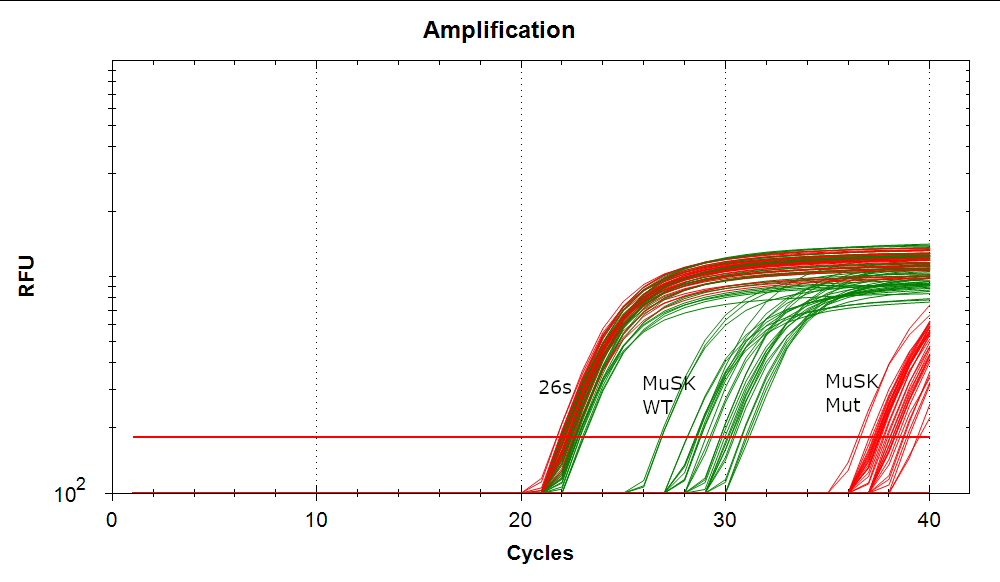
\includegraphics[width=\textwidth]{./Images/qPCR/Amplification.jpg}
			\end{subfigure}
			\begin{subfigure}[h]{0.329\textwidth}
				\caption{}
				\label{fig:qPCRCompaWTMut}
				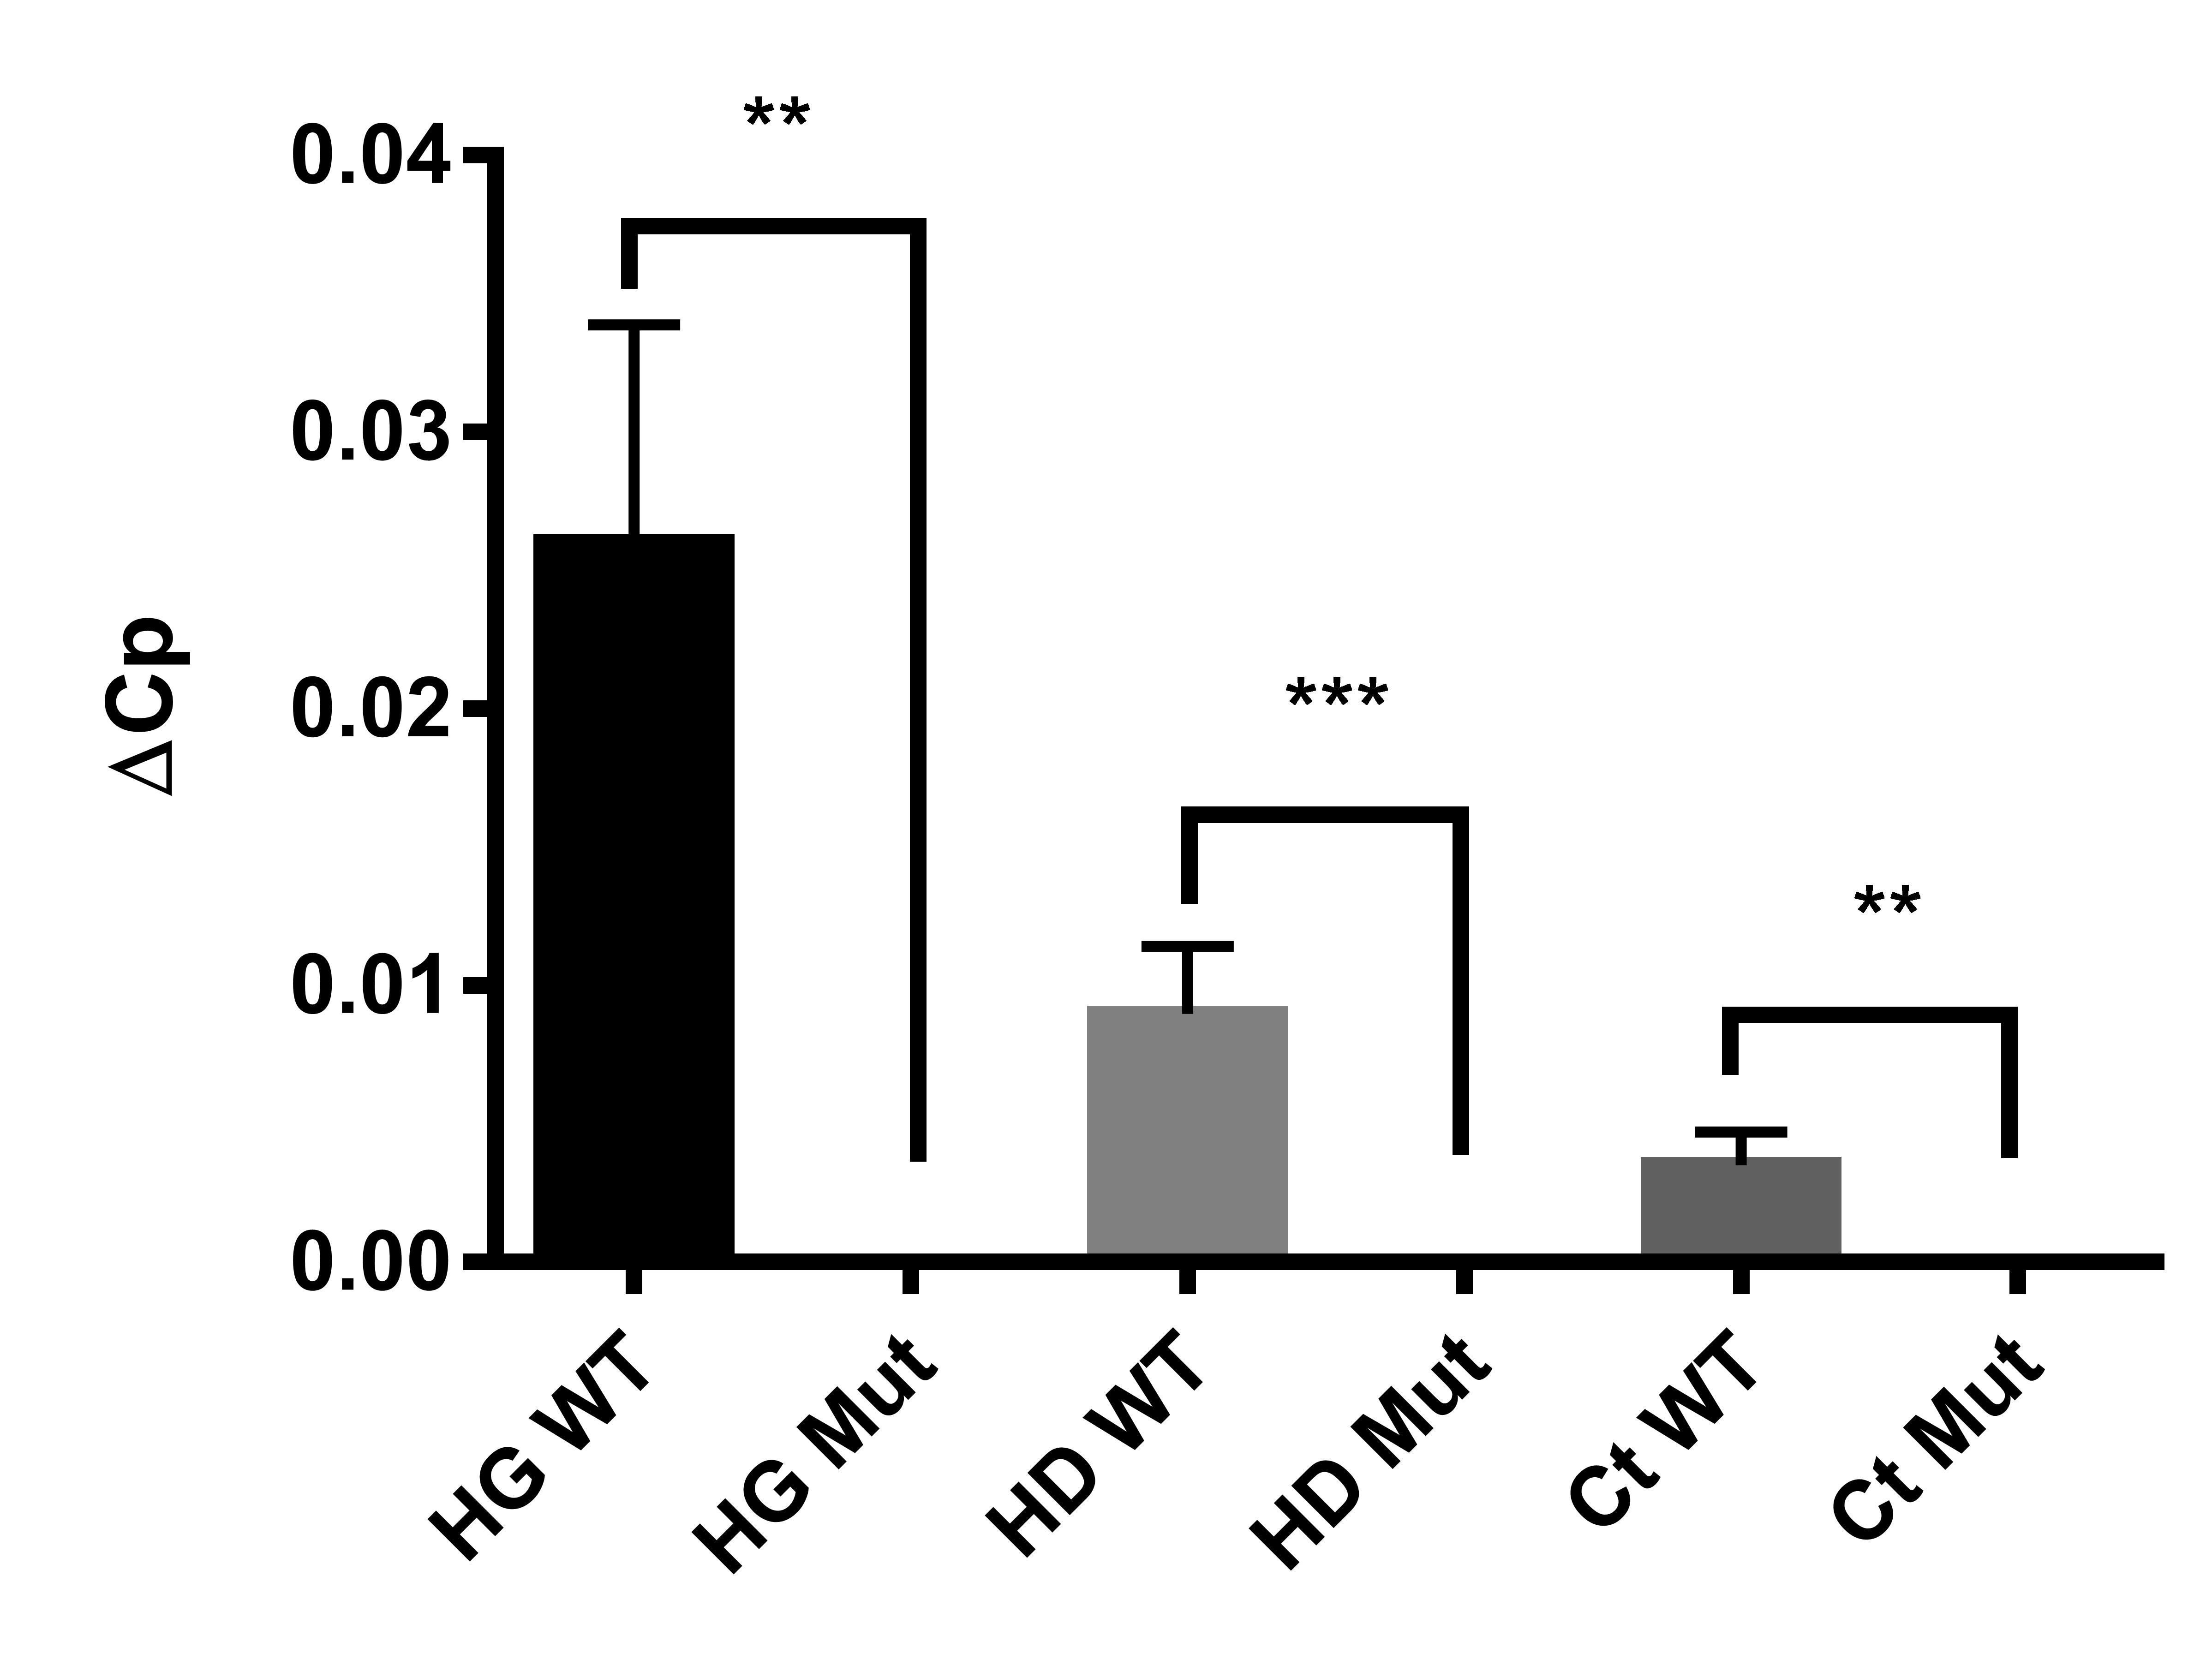
\includegraphics[width=\textwidth]{./Images/qPCR/Comp_WT-Mut.jpg}
			\end{subfigure}
			\begin{subfigure}[h]{0.329\textwidth}
				\caption{}
				\label{fig:qPCRCompaWT}
				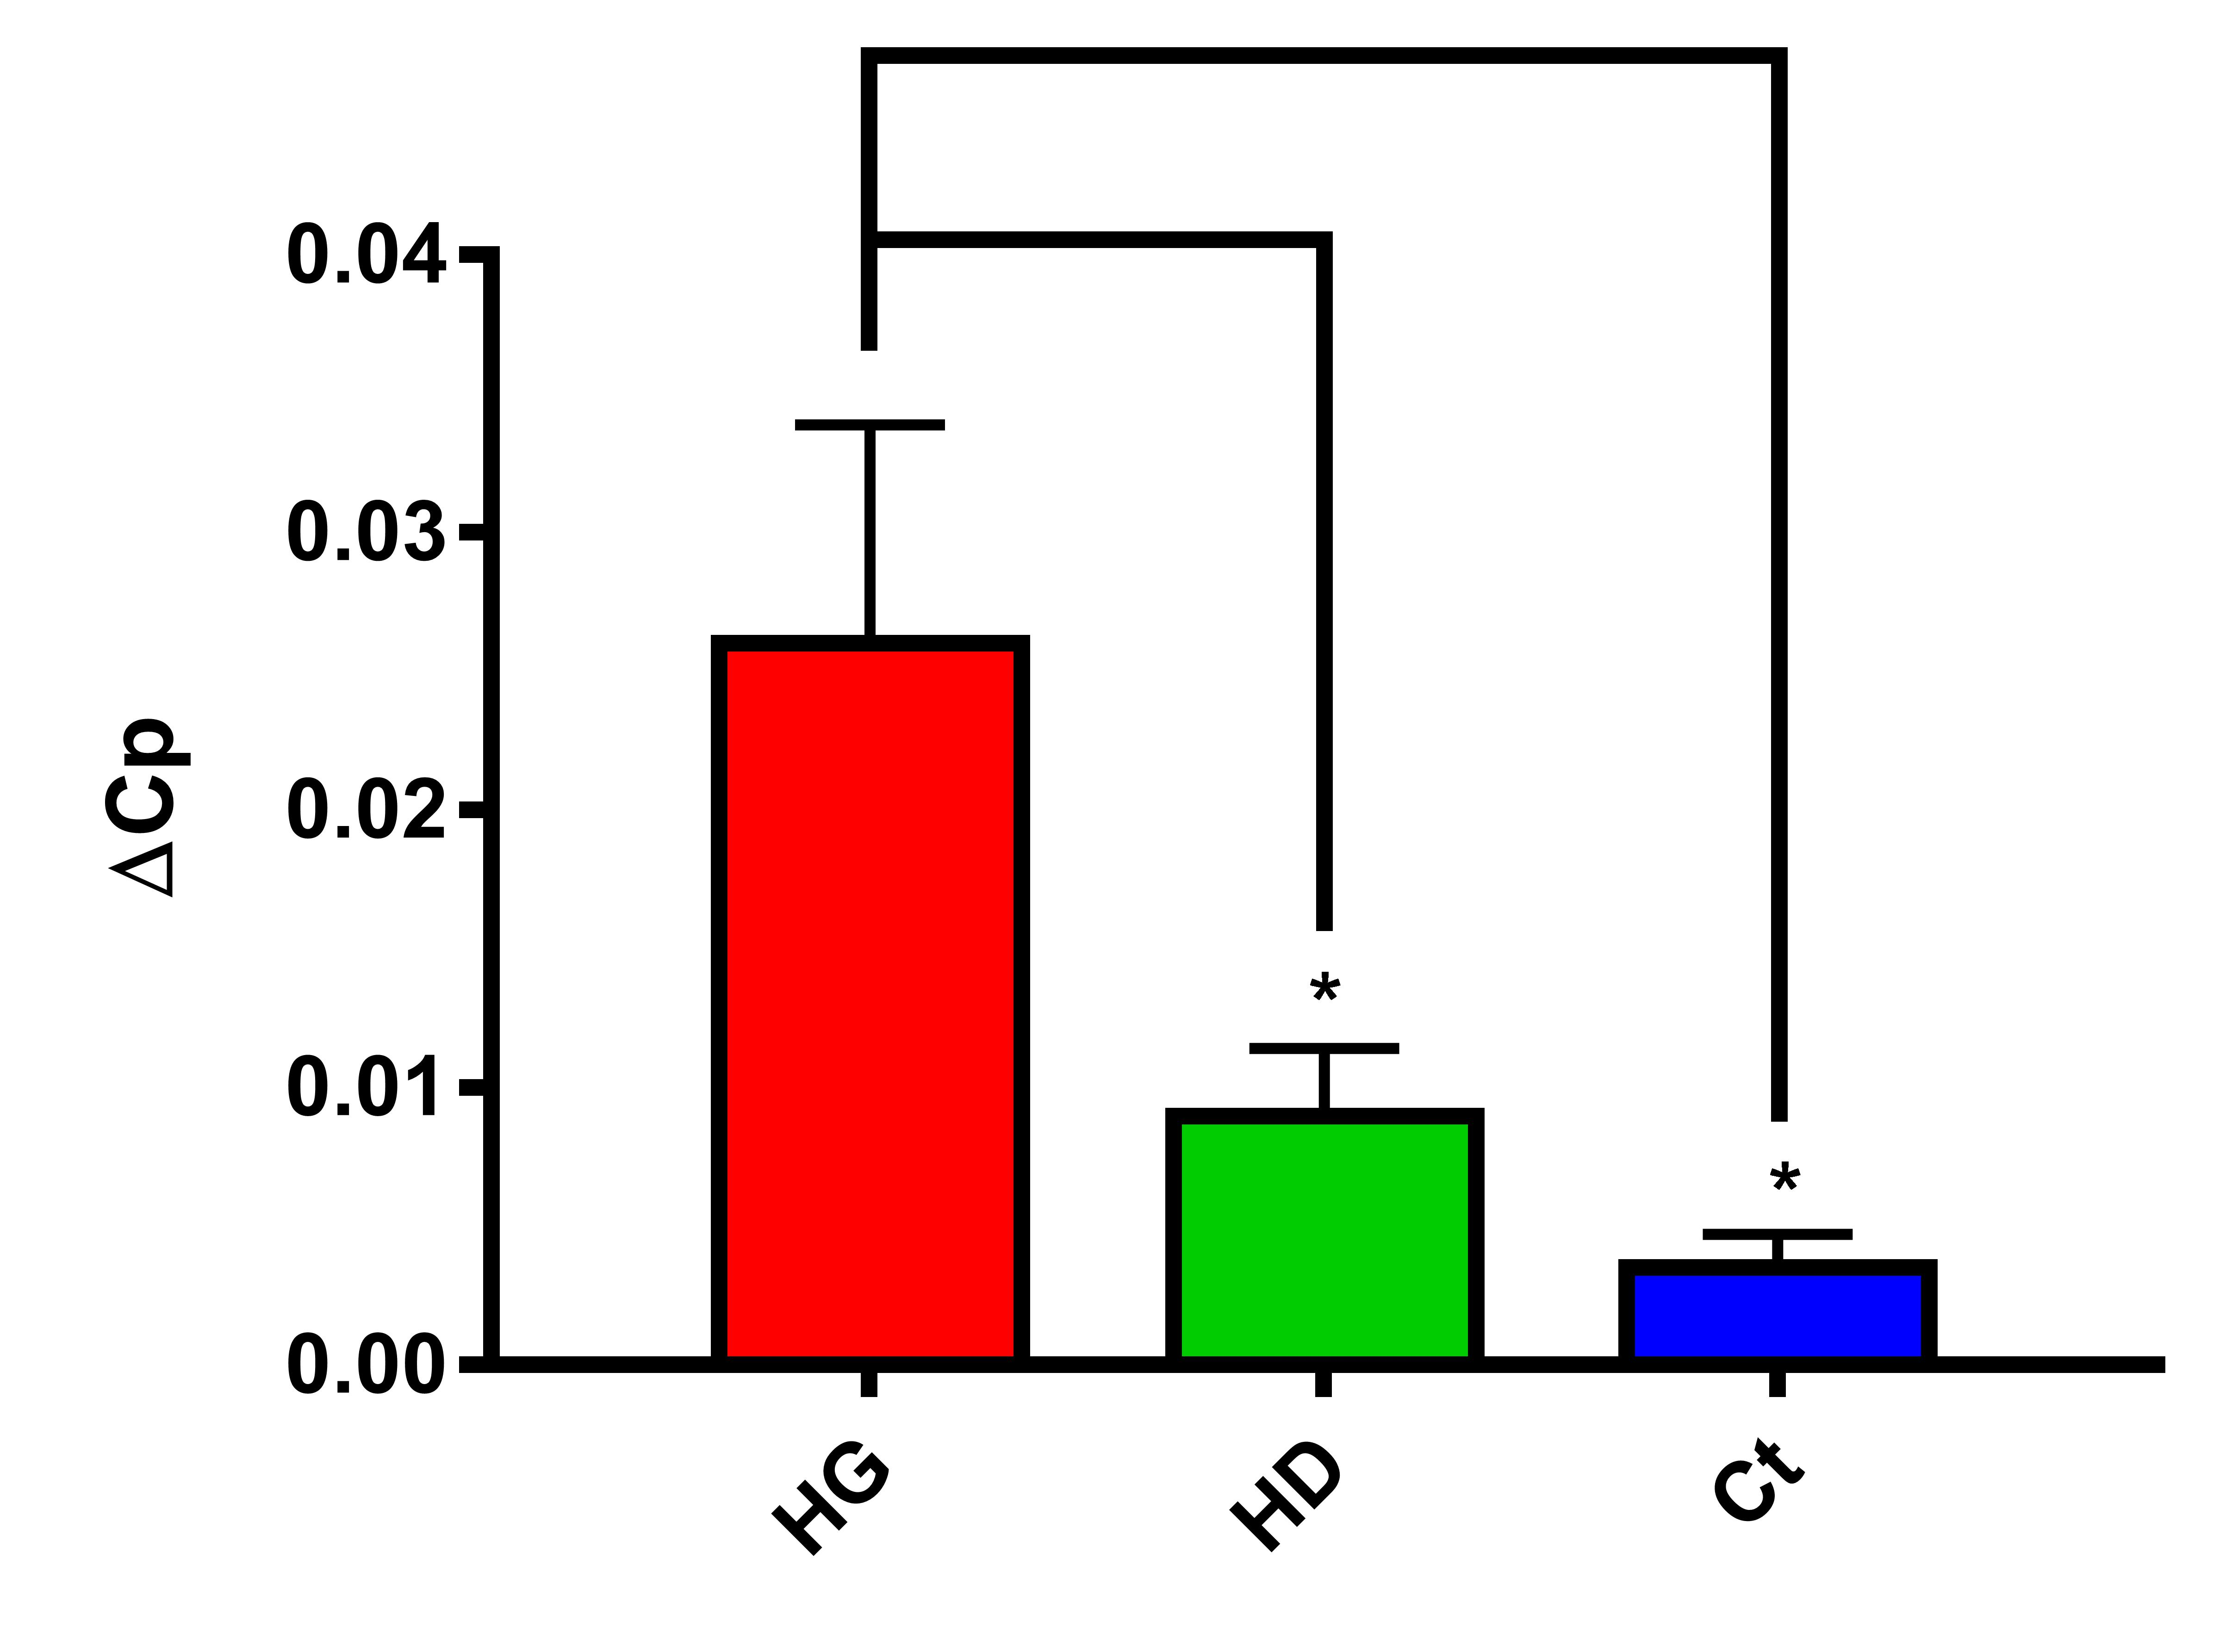
\includegraphics[width=\textwidth]{./Images/qPCR/Comp_Struct_WT.jpg}
			\end{subfigure}
			\begin{subfigure}[h]{0.329\textwidth}
				\caption{}
				\label{fig:qPCRCompaMut}
				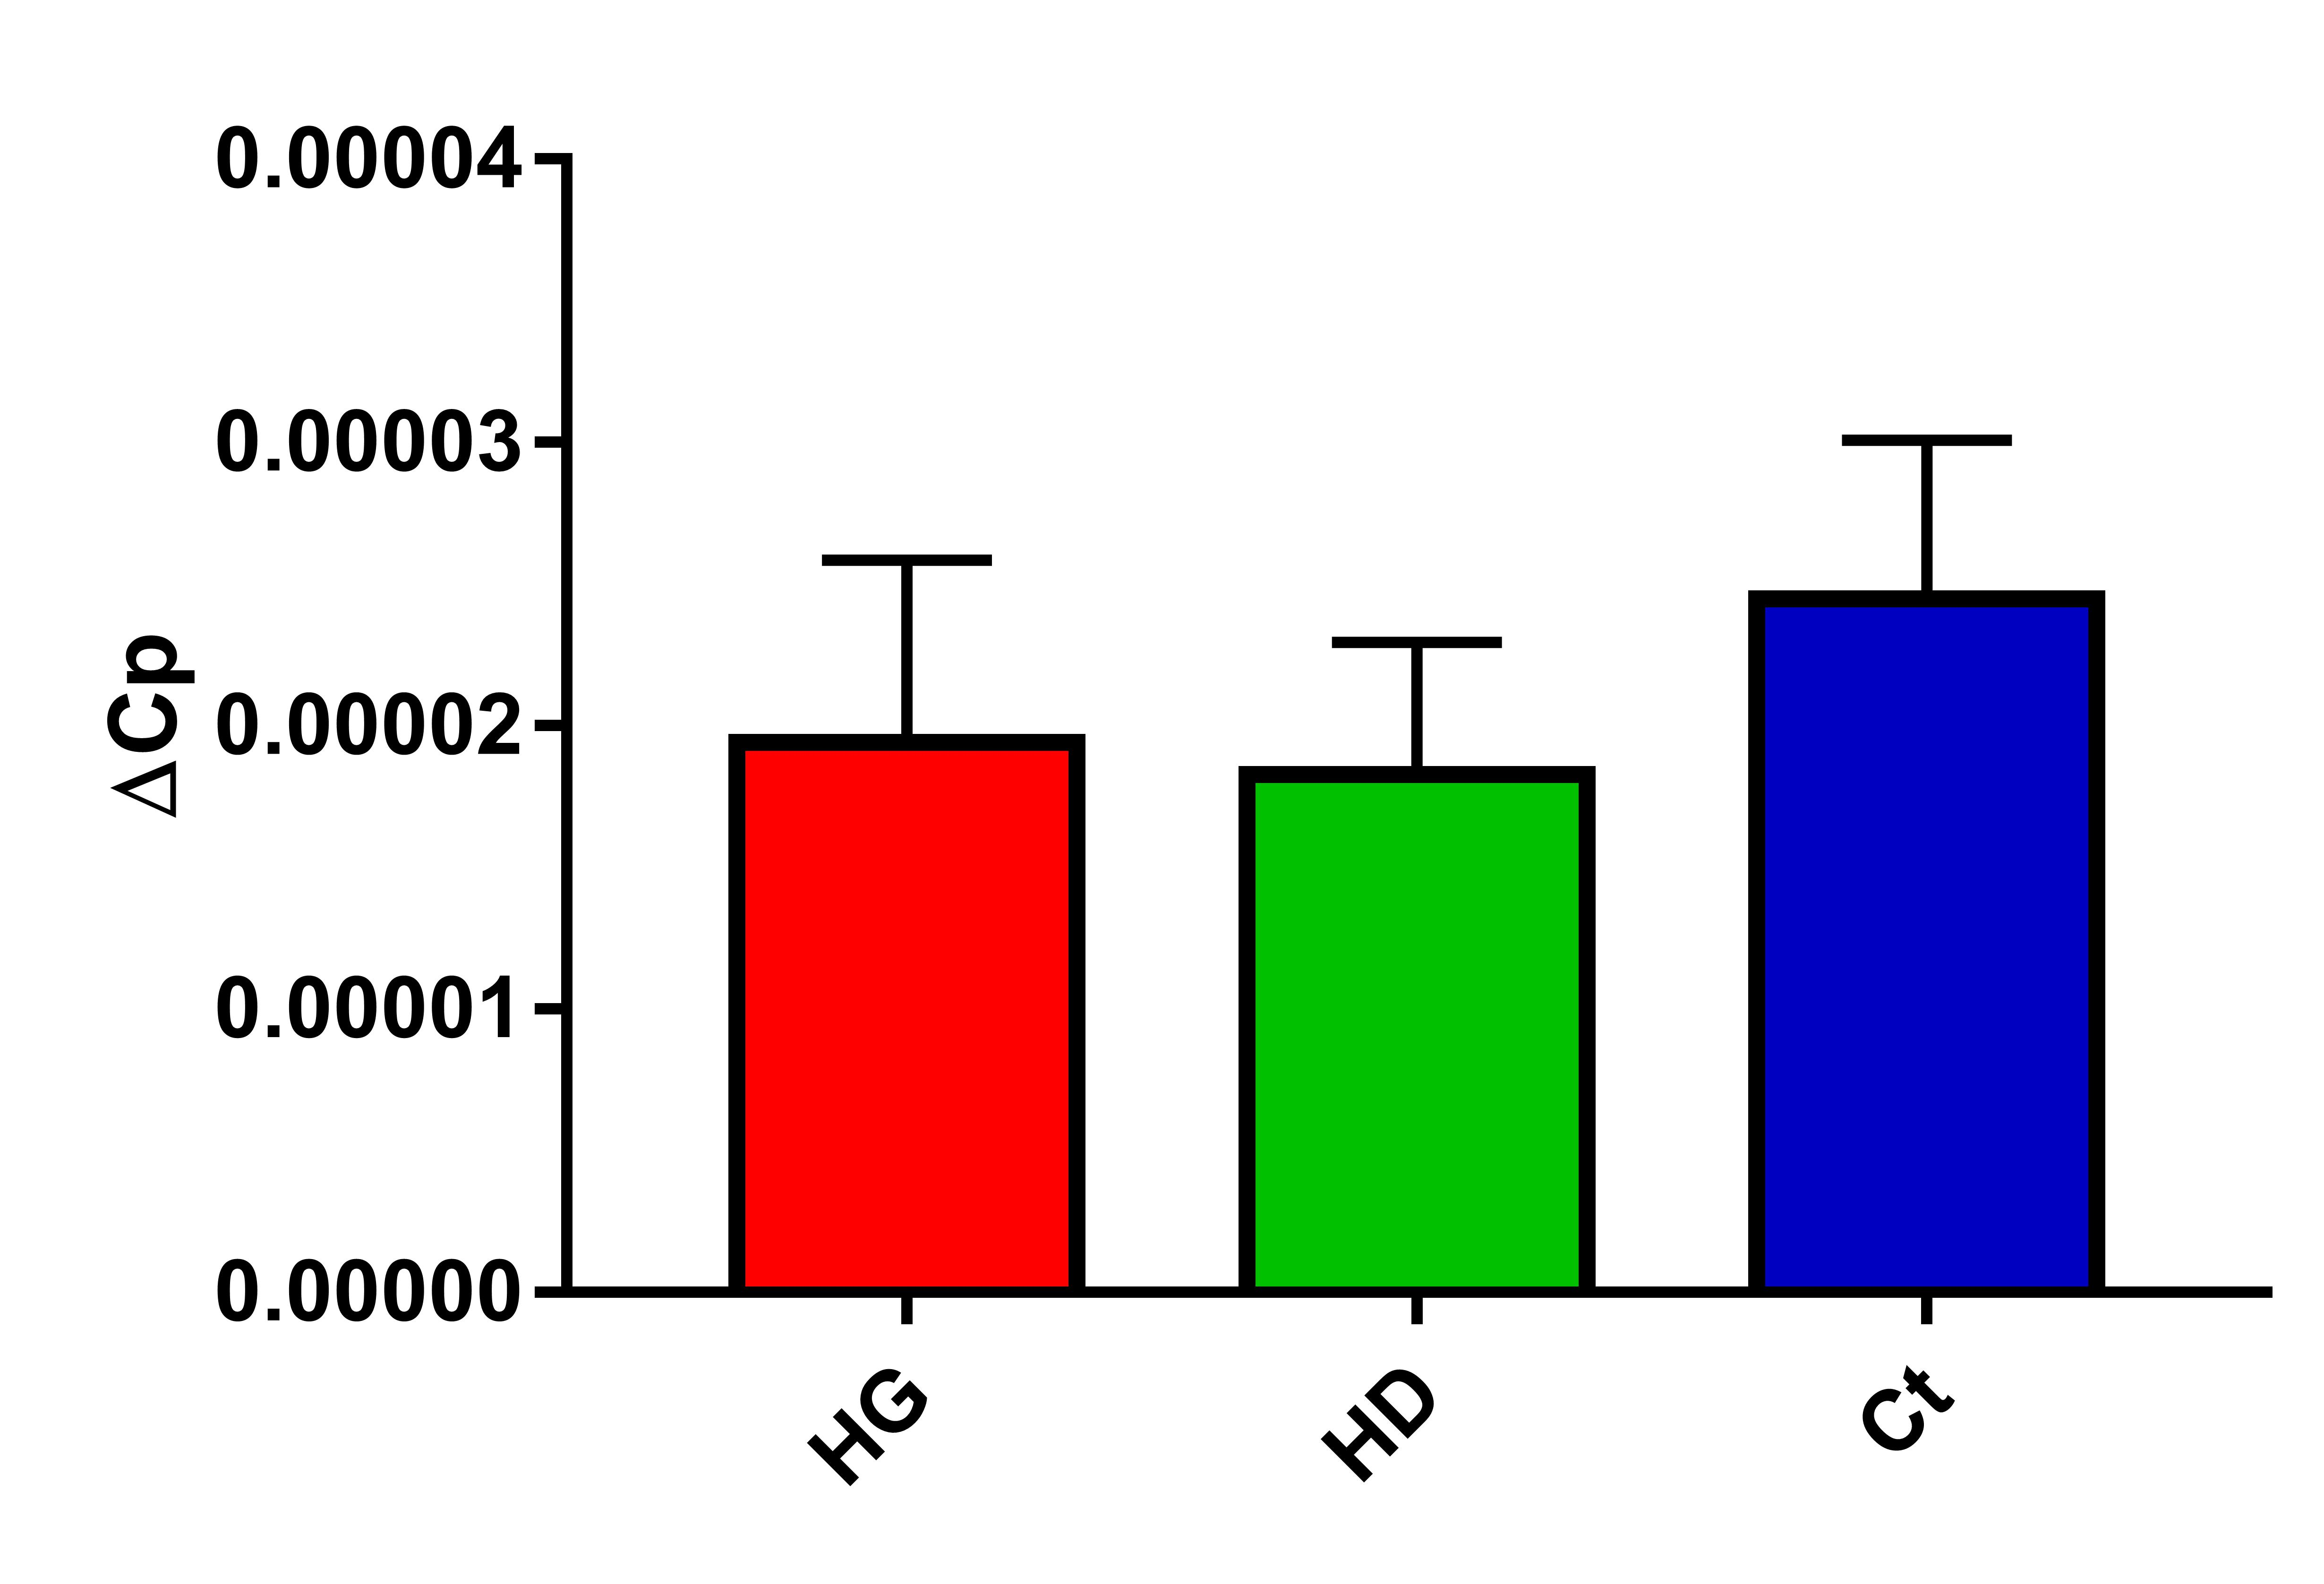
\includegraphics[width=\textwidth]{./Images/qPCR/Comp_Struct_Mut.jpg}
			\end{subfigure}
		\end{center}
		\caption{L'expression de \gls{musk} est fortement diminué chez les mutants.}
		\descfig{%
				\subref{fig:TableAmpli} Comparaison de l'expression \textDelta{}Cp obtenus après normalisation entre des individus \gls{wt} et mutants dans trois structures. Les résultats sont présentés sous la forme moyenne (écart-type).
				\subref{fig:AmpliqPCR} Courbe d'amplification. On peut voir que l'expression du gène de ménage \acrshort{26s} (vers la droite de la courbe) est semblable entre les individus \gls{wt} et \mcrd. Cependant, l'expression de \gls{musk} est grandement diminuée chez les individus mutants (courbes rouges) par rapport aux individus sauvages (courbes vertes).
				\subref{fig:qPCRCompaWTMut} Comparaison de l'expression des différentes structures entre individus sauvages et mutants.
				\subref{fig:qPCRCompaWT} Comparaison de l'expression de \gls{musk} dans différentes structures chez les individus sauvages.
				\subref{fig:qPCRCompaMut} Comparaison de l'expression de \gls{musk} dans différentes structures chez les individus mutants.
				HG : Hippocampe Gauche, HD : Hippocampe Droit, Ct : Cervelet. n = 3 (\gls{wt}) et n = 4 (mutants). Test statistique : Test t de Student non apparié (\subref{fig:qPCRCompaWTMut}), et Test t de Student apparié (\subref{fig:qPCRCompaWT} \& \subref{fig:qPCRCompaMut}). 
				* : p<0.05, ** : p<0.01, *** : p<0.001. 
				}
		\label{fig:ExpressionMuSK}
	\end{figure}
\FloatBarrier
